
\documentclass[a4paper]{scrreprt}
 
\usepackage[german]{babel}
\usepackage[utf8]{inputenc}
\usepackage[T1]{fontenc}
\usepackage{ae}

\usepackage[scaled]{helvet}
\renewcommand\familydefault{\sfdefault} 

\usepackage[onehalfspacing]{setspace}
\usepackage[scaled]{helvet}
\renewcommand*\familydefault{\sfdefault}

\usepackage[T1]{fontenc}
\usepackage{glossaries}
\usepackage{graphicx}
\usepackage[bookmarks,bookmarksnumbered]{hyperref}
\usepackage{float}
\usepackage[font={footnotesize}]{caption}

\setcounter{tocdepth}{1} 
\setcounter{secnumdepth}{2} 

\makenoidxglossaries

\newglossaryentry{Server}
{	name=Server,
	description={Ein Server (englisch server, wörtlich Diener oder Bediensteter, im weiteren Sinn auch Dienst) ist ein Computerprogramm oder ein Computer, der Computerfunktionalitäten wie Dienstprogramme, Daten oder andere Ressourcen bereitstellt, damit andere Computer oder Programme („Clients“) darauf zugreifen können}
}

\newglossaryentry{App}
{ 	name=App,
	plural=Apps,
	description={Als Mobile App (auf Deutsch meist in der Kurzform die App, eine Abkürzung für den Fachbegriff Applikation) wird eine Anwendungssoftware für Mobilgeräte beziehungsweise mobile Betriebssysteme bezeichnet}
}

\newglossaryentry{Nutzer}
{	name=Nutzer,
	description={Ein Benutzer (auch Endbenutzer, Bediener oder kurz Nutzer genannt sowie englisch User) ist eine Person, die ein Hilfs- oder Arbeitsmittel zur Erzielung eines Nutzens verwendet, beispielsweise für eine Zeitersparnis oder Kostensenkung}
}

\newglossaryentry{Desktop Anwendung}
{	name=Desktop Anwendung,
	plural=Desktop Anwendungen,
	description={Als Desktop Anwendungen (auch Anwendungsprogramm, kurz Anwendung oder Applikation; englisch application software, kurz App) werden Computerprogramme bezeichnet, die genutzt werden, um eine nützliche oder gewünschte nicht systemtechnische Funktionalität zu bearbeiten oder zu unterstützen. Sie dienen der „Lösung von Benutzerproblemen“}
}

\newglossaryentry{Drag and Drop}
{	name=Drag and Drop,
	description={Drag and Drop, oft auch Drag’n’Drop, deutsch „Ziehen und Ablegen“, ist eine Methode zur Bedienung grafischer Benutzeroberflächen von Rechnern durch das Bewegen grafischer Elemente mittels eines Zeigegerätes. Ein Element wie z. B. ein Piktogramm kann damit gezogen und über einem möglichen Ziel losgelassen werden. Dieses kann zum Beispiel markierter Text oder das Symbol einer Datei sein }
}

\newglossaryentry{Medikament}
{	name=Medikament,
	description={Arzneimittel oder gleichbedeutend Medikamente (lateinisch medicamentum „Heilmittel“) sind Stoffe oder Stoffzusammensetzungen, die „zur Heilung oder zur Verhütung menschlicher oder tierischer Krankheiten bestimmt sind“ oder sich dazu eignen, physiologische Funktionen zu beeinflussen oder eine medizinische Diagnose zu ermöglichen}
}

\newglossaryentry{NFC}
{ 	name=NFC,
	description={Die Nahfeldkommunikation (Near Field Communication, abgekürzt NFC) ist ein auf der RFID-Technik basierender internationaler Übertragungsstandard zum kontaktlosen Austausch von Daten per elektromagnetischer Induktion mittels loser gekoppelter Spulen über kurze Strecken von wenigen Zentimetern}
}

\newglossaryentry{Versichertennummer}
{ 	name=Versichertennummer,
	description={Die Krankenversichertennummer dient der Identifikation des Versicherten bei einer Krankenversicherung. Die Krankenversichertennummer wird benötigt, damit Leistungserbringer, z. B. Ärzte oder Zahnärzte ihre Leistungen mittels der Krankenversicherungskarte, über die Kassenärztlichen Vereinigungen, mit der zuständigen Krankenkasse abrechnen können}
}


\newglossaryentry{Bluetooth}
{	name=Bluetooth,
	description={Bluetooth ist ein in den 1990er Jahren durch die Bluetooth Special Interest Group (SIG) entwickelter Industriestandard gemäß IEEE 802.15.1 für die Datenübertragung zwischen Geräten über kurze Distanz per Funktechnik (WPAN). Dabei sind verbindungslose sowie verbindungsbehaftete Übertragungen von Punkt zu Punkt und Ad-hoc- oder Piconetze möglich}
}

\newglossaryentry{Pop-Up}
{	name=Pop-Up,
	description={Ein Pop-up (von englisch to pop up, „plötzlich auftauchen“) ist ein Element einer grafischen Benutzeroberfläche. In der Regel werden Pop-ups eingesetzt, um zusätzliche Inhalte anzuzeigen oder eine bestimmte Interaktion abzufragen. Typischerweise „springen“ Pop-ups auf und überdecken dabei andere Teile der Benutzeroberfläche}
}

\newglossaryentry{Cloud}
{	name=Cloud,
	description={Die Cloud ist keine physische Größe, sondern ein riesiges Netzwerk aus Remoteservern, die über die ganzen Welt verteilt aber miteinander verbunden sind, damit sie als ein einziges großes Ökosystem funktionieren können}
}

\newglossaryentry{Tab}
{	name=Tab,
	description={Eine Registerkarte, auch Reiter oder Tab genannt, ist ein Steuerelement einer grafischen Benutzeroberfläche, das einem Registerblatt aus Aktenschränken nachempfunden wurde }
}
 
\newglossaryentry{Arztbrief}
{	name=Arztbrief,
	plural=Arztbriefe,
	description={Der Arztbrief, oft synonym als Epikrise, Entlassungsbrief, Patientenbrief oder Befundbericht bezeichnet, ist ein Transferdokument für die Kommunikation zwischen Ärzten. Der Arztbrief gibt einen zusammenfassenden Überblick über den Status des Patienten bei der Entlassung, einen Rückblick über den Krankheitsverlauf, die veranlasste Therapie, eine Interpretation des Geschehens zum Krankheitsverlauf im speziellen Fall}
}

\newglossaryentry{Anamnese}
{	name=Anamnese,
	description={Die Anamnese (von altgriechisch anámnēsis, deutsch ‚Erinnerung‘) ist die professionelle Erfragung von potenziell medizinisch relevanten Informationen durch Fachpersonal (z. B. einen Arzt)}
}
 
\begin{document}
\begin{titlepage}
\begin{figure}[h]
	\vspace{-4cm}
	\hspace{-2cm}
	
\includegraphics[ width=0.3\textwidth]{Kit_Logo}
	\label{fig:Aufg03_1}
\end{figure}
	\vspace{1.5cm}
	\centering
	
\includegraphics[width=0.5\textwidth]{graphics/myMD_Logo}\par\vspace{0.5cm}
	{\Huge myMD \par}
	\vspace{2cm}
	{\scshape\Large Pflichtenheft\par}
	\vspace{1cm}
	Praxis der Softwareentwicklung WS2017/2018 \par
	\vspace{2cm}
	{\Large\itshape Philipp Pelcz, Philipp Karcher, Jan-Luca Vettel\par}
	\vfill
	supervised by \par
	Marc Aurel Kiefer

	\vfill

% Bottom of the page
	{\large \today \par}
\end{titlepage}
 

% Platzierung des Inhaltsverzeichnisses
\tableofcontents
\addtocontents{toc}{\protect\enlargethispage{10cm}}



\chapter{Zielbestimmung}

\section{Einleitung}
Die digitale Vernetzung aller Lebensbereich dominiert und verändert unseren Alltag seit einigen Jahren wie kaum eine andere Thematik. Viele Branchen erfahren eine sogenannte „digitale Transformation“, die industrielle Produktion soll mittels Industrie 4.0 in das Zeitalter moderner Informationstechnik befördert werden und dank des „Internet der Dinge“ (Internet of Things) kommuniziert eine stetig wachsende Zahl an Alltagsgegenständen über das Internet untereinander, mit dem Ziel, uns das Leben zu erleichtern.\\
Mit dem „E-Health-Gesetz“ hat die Bundesregierung im Jahr 2016 einen Vorstoß unternommen, die digitale Infrastruktur im Gesundheitswesen auszubauen, um so eine der größten Branchen der deutschen Wirtschaft zu digitalisieren.\\
Tatsächlich reicht ein kurzer Blick in die meisten deutschen Arztpraxen oder Krankenhäuser aus, um festzustellen, dass auch heute noch Papier als Speichermedium der Wahl eingesetzt wird. Wenngleich eine große Zahl an Praxen und Kliniken mittlerweile Software zur internen Datenverwaltung einsetzt, so erfolgt die Kommunikation mit dem Patient in den wenigsten Einrichtungen digital.\\
~\\
Im Rahmen der Veranstaltung „Praxis der Softwareentwicklung (PSE)“ und des „Imagine Cup 2018“, einem von Microsoft veranstalteten Wettbewerb, hat es sich unser Team zum Ziel gemacht, dies zu ändern:\\
Mit der Entwicklung von myMD soll es dem Arzt künftig möglich sein, einem Patienten die ihn betreffenden Arztbriefe und Krankenakten in digitaler Form noch im Behandlungszimmer aushändigen zu können. 
Zur selben Zeit ermöglicht myMD es dem Patienten, all seine Patientendaten, Arztbriefe und Krankenakten, die bisher verstreut auf den Computern dutzender Ärzte gesichert waren, an einem Ort zentral gespeichert auf seinem Mobilgerät immer unter Kontrolle zu haben. 

Die Möglichkeiten, um die solch ein System Ärzte und vor allen Dingen Patienten bereichern könnte, reichen von einer naheliegenden Reduktion des Papierverbrauchs in Arztpraxen und Krankenhäusern bis hin zu einer möglichen Minderung gefährlicher Medikamentenwechselwirkungen, an denen jährlich alleine in Deutschland mehrere Zehntausend Menschen sterben.
Der Arzt wäre beispielsweise bei der \gls{Anamnese} nicht alleine auf das Erinnerungsvermögen des Patienten angewiesen, sondern könnte sich mit wenigen Handgriffen ein vollständiges Bild über die Krankengeschichte verschaffen, mögliche Unverträglichkeiten in Erfahrung bringen und aktuellen oder vergangenen Medikamenteneinnahmen studieren, die sich unter Umständen auf die eigene Diagnose und Therapieempfehlung auswirken könnten.
Gleichzeitig könnte myMD den Patienten besser vor überflüssigen Mehrfachuntersuchungen und somit beispielsweise unnötiger Strahlenbelastung schützen, da der Nutzer zu jeder Zeit alle Befunde und Untersuchungsergebnisse auf dem eigenen Mobilgerät bei sich trägt. Ein weiterer wichtiger Aspekt ist hierbei die zeitlich unbegrenzte Archivierung der gespeicherten Gesundheitsinformationen, denn im Gegensatz zur gesetzlich vorgeschriebenen Mindestspeicherdauer von 10 Jahren kann der Patient mit myMD selbst entscheiden, ob und wann er Einträge von seinem Mobilgerät entfernen möchte. Gerade für Krebspatienten, die neben der Datenvollständigkeit häufig auch mit enormen Papier- und Aktenbergen zu kämpfen haben, wäre dies eine hilfreiche Unterstützung.

 
\section{Pflichtkriterien (PK)}
\subsection{Patientenseitige Datenübertragung}
\begin{tabular}{lll}

[PK1010] & \multicolumn{2}{p{12cm}}  {\glspl{Arztbrief} können von der \gls{Desktop Anwendung} auf die myMD \gls{App} des Patienten übertragen werden.} \\
{[PK1020]} & \multicolumn{2}{p{12cm}}  {Die Übertragung erfolgt verschlüsselt über \gls{Bluetooth}.} \\
{[PK1030]} & \multicolumn{2}{p{12cm}}  {Eine laufende Datenübertragung kann manuell abgebrochen werden.} \\

\end{tabular}

\subsection{Darstellung}
\begin{tabular}{lll}
[PK2010] & \multicolumn{2}{p{12cm}}  {\glspl{Arztbrief} werden chronologisch absteigend im \gls{Tab} \textit{Übersicht} dargestellt.} \\
{[PK2020]} & \multicolumn{2}{p{12cm}}  {Der \gls{Nutzer} kann überflüssige/unerwünschte \glspl{Arztbrief} löschen.} \\
{[PK2030]} & \multicolumn{2}{p{12cm}}  {Die Darstellung eines Arztbriefes umfasst die Diagnose, verordnete \gls{Medikament}e, das Datum und den Namen des behandelnden Arztes.} \\
\end{tabular}

\subsection{Einstellungen}
\begin{tabular}{lll}
[PK3010] & \multicolumn{2}{p{12cm}}  {Der \gls{Nutzer} kann ein eigenes Profil anlegen, welches Daten wie den Namen, Versicherungsnummer, Blutgruppe und Allergien enthält.} \\
{[PK3020]} & \multicolumn{2}{p{12cm}}  {Die myMD \gls{App} wird in Deutsch angeboten.} \\

\end{tabular}

\subsection{\gls{Desktop Anwendung}}
\begin{tabular}{lll}
{[PK4010]} & \multicolumn{2}{p{12cm}}  {Die \gls{Desktop Anwendung} kann die Geräte in der Nähe anzeigen.} \\
{[PK4020]} & \multicolumn{2}{p{12cm}}  {Der Arzt kann unter den Geräten in der Nähe das Mobilgerät des Patienten als Empfänger auswählen.} \\
{[PK4030]} & \multicolumn{2}{p{12cm}}  {Digitale \glspl{Arztbrief} können entweder per \gls{Drag and Drop} oder über einen Explorer in die \gls{Desktop Anwendung} geladen werden.} \\
{[PK4040]} & \multicolumn{2}{p{12cm}}  {Die Daten werden auf Knopfdruck an das Mobilgerät des Patienten gesendet.} \\
\end{tabular}

\subsection{Kompatibilität}
\begin{tabular}{lll}
[PK5010] & \multicolumn{2}{p{12cm}}  {Die \gls{Desktop Anwendung} wird von Microsoft Windows 10 unterstützt.} \\
{[PK5020]} & \multicolumn{2}{p{12cm}}  {Die myMD \gls{App} wird von Android 6.0 (und höher) unterstützt.} \\
{[PK5030]} & \multicolumn{2}{p{12cm}}  {Die myMD \gls{App} kann \glspl{Arztbrief} im .hl7 Dateiformat anzeigen.} \\

\end{tabular}
 
\section{Wunschkriterien (WK)}
\subsection{Patientenseitige Datenübertragung}
\begin{tabular}{lll}
[WK1010] & \multicolumn{2}{p{12cm}}  {Ein \gls{Arztbrief} kann von der myMD \gls{App} des Patienten auf die \gls{Desktop Anwendung} übertragen werden.} \\
{[WK1020]} & \multicolumn{2}{p{12cm}}  {Der Patient kann mehrere \glspl{Arztbrief} gleichzeitig senden.} \\
{[WK1030]} & \multicolumn{2}{p{12cm}}  {\gls{NFC} steht als weitere Übertragungsmöglichkeit zur Verfügung.} \\
{[WK1040]} & \multicolumn{2}{p{12cm}}  {Der Patient wird vor dem Senden von sensiblen Daten darauf hingewiesen, dass er sensible Daten versendet.} \\
{[WK1050]} & \multicolumn{2}{p{12cm}}  {Ein Profil auf einem Mobilgerät kann auf ein anderes übertragen werden.} \\

\end{tabular}

\subsection{Darstellung}
\begin{tabular}{lll}
[WK2010] & \multicolumn{2}{p{12cm}}  {Eingenommene \gls{Medikament}e werden in einem extra \gls{Tab} chronologisch absteigend sortiert dargestellt.} \\
{[WK2020]} & \multicolumn{2}{p{12cm}}  {Laborwerte des Patienten werden in einem extra \gls{Tab} chronologisch absteigend sortiert dargestellt.} \\
{[WK2030]} & \multicolumn{2}{p{12cm}}  {Ein \gls{Arztbrief} kann Bilddateien enthalten und die myMD \gls{App} kann diese originalgetreu darstellen und einem \gls{Arztbrief} zuordnen.} \\
{[WK2040]} & \multicolumn{2}{p{12cm}}  {Es gibt die Möglichkeit, \glspl{Arztbrief} nach eigenen Kriterien (Arzt, Krankheit o.ä.) zu gruppieren.} \\
{[WK2050]} & \multicolumn{2}{p{12cm}}  {Es gibt eine Suchfunktion, die alle \glspl{Arztbrief} nach Daten durchsucht.} \\
\end{tabular}

\subsection{Einstellungen}
\begin{tabular}{lll}
[WK3010] & \multicolumn{2}{p{12cm}}  {Auf einer myMD \gls{App} können mehrere \gls{Nutzer} verwaltet werden.} \\
{[WK3020]} & \multicolumn{2}{p{12cm}}  {Die myMD \gls{App} wird zusätzlich auch auf Englisch angeboten.} \\
{[WK3030]} & \multicolumn{2}{p{12cm}}  {Der \gls{Nutzer} kann einzelne \glspl{Arztbrief} oder ganze Gruppen als sensibel markieren.} \\
{[WK3040]} & \multicolumn{2}{p{12cm}}  {Die myMD \gls{App} kann den \gls{Nutzer} an regelmäßige Arzttermine (z.B. Zahnarzt, Augenarzt) erinnern.} \\

\end{tabular}

\subsection{\gls{Desktop Anwendung}}
\begin{tabular}{lll}

{[WK4010]} & \multicolumn{2}{p{12cm}}  {Die \gls{Versichertennummer}, die in einem \gls{Arztbrief} auf dem Computer des Arztes eingetragen ist, wird vor dem Senden mit der in der myMD App des Patienten hinterlegten \gls{Versichertennummer} abgeglichen und nur bei Übereinstimmung wird der \gls{Arztbrief} gesendet.} \\

\end{tabular}

\subsection{Kompatibilität}
\begin{tabular}{lll}
{[WK5010]} & \multicolumn{2}{p{12cm}}  {Die myMD \gls{App} wird von iOS 10 (und höher) unterstützt.} \\
{[WK5020]} & \multicolumn{2}{p{12cm}}  {Die \gls{Desktop Anwendung} wird zusätzlich von macOS 10.12 (und höher) unterstützt.} \\
{[WK5030]} & \multicolumn{2}{p{12cm}}  {Die myMD \gls{App} kann \gls{Arztbrief}e im .pdf Dateiformat anzeigen.} \\
{[WK5040]} & \multicolumn{2}{p{12cm}}  {Die myMD \gls{App} kann \gls{Arztbrief}e im .csv Dateiformat anzeigen.} \\

\end{tabular}
 
\section{Abgrenzungskriterien (AK)}
\begin{tabular}{ll}

[AK0010] &  Die Anwendung selbst stellt keine medizinischen Diagnosen. \\
{[AK0020]} &  Es werden keine Daten auf einem \gls{Server} oder in einer \gls{Cloud} gespeichert. \\
{[AK0030]} &  Die Anwendung stellt keinen Ersatz zu einem Arzttermin dar. \\
{[AK0040]} &  Die Anwendung stellt keinen Ersatz zu einer Versichertenkarte dar. \\
{[AK0050]} &  Es gibt keine Möglichkeit zur Terminvereinbarung. \\
{[AK0060]} &  Der \gls{Nutzer} kann einen \gls{Arztbrief} nicht editieren. \\

\end{tabular}
 
\chapter{Produkteinsatz}

\section{Einsatzgebiete}
In vielen Situationen kann myMD zum Einsatz kommen, zwei sind dabei besonders charakteristisch: \newline
Zum einen kann die App immer eine wichtige Unterstützung sein, wenn der \gls{Nutzer} sich einen Überblick über die eigene Krankheitshistorie verschaffen möchte, 
zum anderen spielt myMD dann eine große Rolle, wenn Ärzte sich einen möglichst lückenlosen Überblick über den Patienten verschaffen müssen.

\section{Produktumgebung}
\begin{tabular}{lll}
\textbf{{Betriebssystem}} & \multicolumn{2}{p{11.5cm}}  {Auf dem Mobilgerät des Patienten muss Android 6.0 (oder höher) installiert sein.}\\
{} & \multicolumn{2}{p{11.5cm}} {Auf dem Computer des Arztes muss Windows 10 installiert sein.} \\
\end{tabular} 

\section{Betriebsbedingungen}
{\textbf{Um die korrekte Übertragung digitaler \glspl{Arztbrief} zu gewährleisten, müssen folgende Bedingungen erfüllt sein:}} \newline\newline
\begin{tabular}{lll}
\textbf{\gls{Bluetooth}} & \multicolumn{2}{p{11.5cm}}{Sowohl das Mobilgerät des Patienten, als auch der Computer des Arztes müssen mindestens über \gls{Bluetooth} 4.0 Low Energy verfügen.} \\
\end{tabular} 
 
\section{Zielgruppen}
Die Anwendung richtet sich an zwei verschiedene Zielgruppen:  \\\\
\begin{tabular}{lll}
\textbf{Patienten} &  \multicolumn{2}{p{12cm}}{Dies sind alle Menschen, die momentan oder in der Vergangenheit eine medizinische Behandlung oder Beratung in Anspruch nehmen oder genommen haben. Ihr Ziel ist es, alle Daten darüber auf ihrem Mobilgerät verwalten und einsehen zu können.}\\
\textbf{Ärzte} &  \multicolumn{2}{p{12cm}}{Diese bieten medizinische Behandlung und Beratung an. Die Anwendung erlaubt es ihnen, alle relevanten medizinischen Daten über einen Patienten von diesem zu erhalten und ihm selbst erstellte Daten zu übermitteln.}  \\
\end{tabular}

\chapter{Produktfunktionen}

\section{Grundfunktionen (GF)}
\subsection{Patientenseitige Datenübertragung}
\begin{tabular}{lll}
[GF1010]&  \multicolumn{2}{p{12cm}}{Die \gls{Desktop Anwendung} sendet einen \gls{Arztbrief} an die myMD \gls{App} [PK1010].}\\
{[GF1020]} &  \multicolumn{2}{p{12cm}}{Verschlüsselte Übertragung der Daten [PK1020].}  \\
{[GF1030]} &  \multicolumn{2}{p{12cm}}{Lokale, drahtlose Übertragung der Daten [PK1020].}  \\
{[GF1040]} &  \multicolumn{2}{p{12cm}}{Übertragung kann bei Bedarf abgebrochen werden [PK1030].}  \\
\end{tabular}

\subsection{Darstellung}
\begin{tabular}{lll}
{[GF2010]}&  \multicolumn{2}{p{12cm}}{Im \gls{Tab} \textit{Übersicht} werden alle geladenen \glspl{Arztbrief} aufgelistet [PK2010].} \\
{[GF2020]} &  \multicolumn{2}{p{12cm}}{Löschen einzelner \glspl{Arztbrief} [PK2020].}  \\
{[GF2030]} &  \multicolumn{2}{p{12cm}}{Der digitale \gls{Arztbrief} zeigt die ausgestellte Diagnose an [PK2030].}  \\
{[GF2040]} &  \multicolumn{2}{p{12cm}}{Der digitale \gls{Arztbrief} zeigt die verschriebenen \gls{Medikament}e an [PK2030].}  \\
{[GF2050]} &  \multicolumn{2}{p{12cm}}{Der digitale \gls{Arztbrief} zeigt das Erstellungsdatum des Artztbriefes an [PK2030].}  \\
{[GF2060]} &  \multicolumn{2}{p{12cm}}{Der digitale \gls{Arztbrief} zeigt den Namen des Arztes an [PK2030].}  \\
{[GF2070]} &  \multicolumn{2}{p{12cm}}{Der digitale \gls{Arztbrief} wird im \gls{Tab} \textit{Übersicht} kompakt dargestellt.}  \\
{[GF2080]} &  \multicolumn{2}{p{12cm}}{Tippen auf einen Listeneintrag im \gls{Tab} \textit{Übersicht} öffnet eine ausführliche Ansicht des Arztbriefes.}  \\
\end{tabular}

\subsection{Einstellungen}
\begin{tabular}{lll}
[GF3010]&  \multicolumn{2}{p{12cm}}{Anlegen eines Nutzerprofils [PK3010].}\\
{[GF3020]} &  \multicolumn{2}{p{12cm}}{Hinzufügen des Vor-/Nachnamens zum Nutzerprofil [PK3010].}  \\
{[GF3030]} &  \multicolumn{2}{p{12cm}}{Hinzufügen der \gls{Versichertennummer} zum Nutzerprofil [PK3010].}  \\
{[GF3040]} &  \multicolumn{2}{p{12cm}}{Hinzufügen der Blutgruppe zum Nutzerprofil [PK3010].}  \\
{[GF3050]} &  \multicolumn{2}{p{12cm}}{Hinzufügen eines Profilbildes zum Nutzerprofil [PK3010].}  \\
\end{tabular}

\subsection{\gls{Desktop Anwendung}}
\begin{tabular}{lll}
[GF4010]&  \multicolumn{2}{p{12cm}}{Kompatible Geräte in Reichweite werden aufgelistet [PK4010],[PK5010],[PK5020],[WK5010],[WK5020].}\\
{[GF4020]} &  \multicolumn{2}{p{12cm}}{Kompatible Dateien können in die \gls{Desktop Anwendung} geladen werden [PK4030],[PK5030],[WK5030].}  \\
{[GF4030]} &  \multicolumn{2}{p{12cm}}{Verbindungsaufbau zum Mobilgerät des Patienten [PK4020].}  \\
{[GF4040]} &  \multicolumn{2}{p{12cm}}{Senden der Datei/en [PK4040].}  \\
\end{tabular}

\section{Optionale Funktionen (OF)}

\subsection{Patientenseitige Datenübertragung}
\begin{tabular}{lll}
[OF1010]&  \multicolumn{2}{p{12cm}}{Die myMD \gls{App} sendet einen \gls{Arztbrief} an die \gls{Desktop Anwendung} [WK1010].}\\
{[OF1020]} &  \multicolumn{2}{p{12cm}}{Das Senden von mehreren Arztbriefen wird unterstützt [WK1020].}  \\
{[OF1030]} &  \multicolumn{2}{p{12cm}}{Der Verbindungsaufbau (ggf. auch die Übertragung) erfolgt über \gls{NFC} [WK1030].}  \\
{[OF1040]} &  \multicolumn{2}{p{12cm}}{Es wird erkannt, dass der \gls{Nutzer} sensible Daten senden will, woraufhin er nochmals durch ein \gls{Pop-Up} benachrichtigt wird [WK1040].}  \\
{[OF1050]} &  \multicolumn{2}{p{12cm}}{Ein Profil kann auf ein anderes Mobilgerät exportiert werden [WK1050].}  \\

\end{tabular}

\subsection{Darstellung}
\begin{tabular}{lll}
[OF2010]&  \multicolumn{2}{p{12cm}}{\gls{Medikament}e werden in einem eigenen \gls{Tab} dargestellt [WK2010].}\\
{[OF2020]}&  \multicolumn{2}{p{12cm}}{\gls{Medikament}e werden chronologisch absteigend sortiert [WK2010].}\\
{[OF2030]}&  \multicolumn{2}{p{12cm}}{Laborwerte werden in einem eigenen \gls{Tab} dargestellt [WK2020].}\\
{[OF2040]}&  \multicolumn{2}{p{12cm}}{Laborwerte werden chronologisch absteigend sortiert [WK2020].}\\
{[OF2030]} &  \multicolumn{2}{p{12cm}}{Bilddateien werden beim Senden zugelassen [WK2030].}  \\
{[OF2040]} &  \multicolumn{2}{p{12cm}}{Bilddateien (z.B. Röntgenbilder) können manuell zu einem passenden \gls{Arztbrief} zugeordnet werden [WK2030].}  \\
{[OF2050]} &  \multicolumn{2}{p{12cm}}{Eine Bilddatei wird originalgetreu dargestellt [WK2030].}  \\
{[OF2060]} &  \multicolumn{2}{p{12cm}}{Arztbriefe können nach eigenen Kriterien gruppiert werden [WK2040].}  \\
{[OF2070]} &  \multicolumn{2}{p{12cm}}{Sortierung nach eigenen Gruppen [WK2040].}  \\
{[OF2080]} &  \multicolumn{2}{p{12cm}}{Der \gls{Nutzer} kann seine Daten nach Schlagworten durchsuchen [WK2050].}  \\

\end{tabular}

\subsection{Einstellungen}
\begin{tabular}{lll}
[OF3010] &  \multicolumn{2}{p{12cm}}{Zusätzliche \gls{Nutzer}profile können hinzugefügt werden [WK3010].}\\
{[OF3020]} &  \multicolumn{2}{p{12cm}}{Man kann zwischen den Nutzerprofilen wechseln [WK3010].}\\
{[OF3030]} &  \multicolumn{2}{p{12cm}}{Man kann Nutzerprofile löschen [WK3010].}\\
{[OF3040]} &  \multicolumn{2}{p{12cm}}{Einzelne oder Gruppen von \glspl{Arztbrief}n können mit einer Sensibilitätswertung versehen werden [WK3030].}  \\
{[OF3050]} &  \multicolumn{2}{p{12cm}}{Hinzufügen von regelmäßigen Arztterminen [WK3040].}  \\
{[OF3060]} &  \multicolumn{2}{p{12cm}}{Löschen von regelmäßigen Arztterminen [WK3040].}  \\
\end{tabular}

\subsection{\gls{Desktop Anwendung}}
\begin{tabular}{lll}
{[OF4010]}&  \multicolumn{2}{p{12cm}}{Die Anwendung verhindert das Senden an eine myMD \gls{App}, falls die \gls{Versichertennummer} im \gls{Arztbrief} nicht mit der \gls{Versichertennummer} im Profil der myMD App übereinstimmt [WK4010].}\\
\end{tabular}
\newpage
\section{Produktleistungen (PL)}
Bei einer drahtlosen Datenübertragung haben viele externe Faktoren, beispielsweise die Signalstärke oder mögliche Interferenzen von anderen Geräten, große Auswirkungen auf Eigenschaften wie die Übertragungsgeschwindigkeit. Diese externen Einflüsse lassen sich auch mit Software nicht oder nur geringfügig korrigieren, weshalb an dieser Stelle keine Aussagen über die Dauer einer Übertragung oder ähnliches getroffen werden.

\stepcounter{subsection}

\subsection{Darstellung}
\begin{tabular}{lll}
[PL2010]&  \multicolumn{2}{p{12cm}}{Zwischen dem Ende der Übertragung eines digitalen Arztbriefes und dem Anzeigen des neuen Eintrages vergehen nicht mehr als 5 Sekunden.}\\
{[PL2020]}&  \multicolumn{2}{p{12cm}}{Die Dauer zwischen dem Tippen auf einen Eintrag in der Ansicht Übersicht und dem Anzeigen des detaillierten Arztbriefes beträgt nicht mehr als 3 Sekunden.}\\

\end{tabular}

\subsection{Einstellungen}
\begin{tabular}{lll}
[PL3010]&  \multicolumn{2}{p{12cm}}{Das Starten der myMD App dauert auf einem aktuellen Mobilgerät nicht länger als 10 Sekunden.}\\


\end{tabular}

\subsection{\gls{Desktop Anwendung}}
\begin{tabular}{lll}
[PL4010]&  \multicolumn{2}{p{12cm}}{Das Starten des myMD Desktop Klienten dauert auf einem aktuellen Computer nicht länger als 5 Sekunden.}\\

\end{tabular}



\chapter{Produktdaten}
\subsection{myMD \gls{App}}
myMD speichert folgende Daten permanent, außer der \gls{Nutzer} löscht sie manuell. Außerdem werden die Daten, die myMD nutzt, ausschließlich lokal auf dem Mobilgerät des Nutzers gespeichert.
\newline
\newline
\begin{tabular}{lll}
[PD1010]&  \multicolumn{2}{p{12cm}}{myMD speichert digitale \glspl{Arztbrief} des Nutzers.}\\
{[PD1020]} &  \multicolumn{2}{p{12cm}}{myMD speichert die Angaben zum Nutzerprofil.}\\
{[PD1030]} &  \multicolumn{2}{p{12cm}}{myMD speichert die Laborwerte des Nutzers.}\\
{[PD1040]} &  \multicolumn{2}{p{12cm}}{myMD speichert die \gls{Medikament}e des Nutzers.}  \\
{[PD1050]} &  \multicolumn{2}{p{12cm}}{myMD speichert regelmäßige Termine des Nutzers.}  \\
{[PD1060]} &  \multicolumn{2}{p{12cm}}{myMD speichert die Einstellungen zu den nutzerspezifischen Gruppierungen.}  \\
{[PD1070]} &  \multicolumn{2}{p{12cm}}{myMD speichert die Markierung von sensiblen Daten.}  \\

\end{tabular}

\subsection{\gls{Desktop Anwendung}}
Die \gls{Desktop Anwendung} speichert den Namen und Fachrichtung des Arztes (diese werden beim Setup manuell eingetragen).


\chapter{Systemmodelle}
\section{Systemarchitektur}
\begin{figure}[ht]
  \centering
  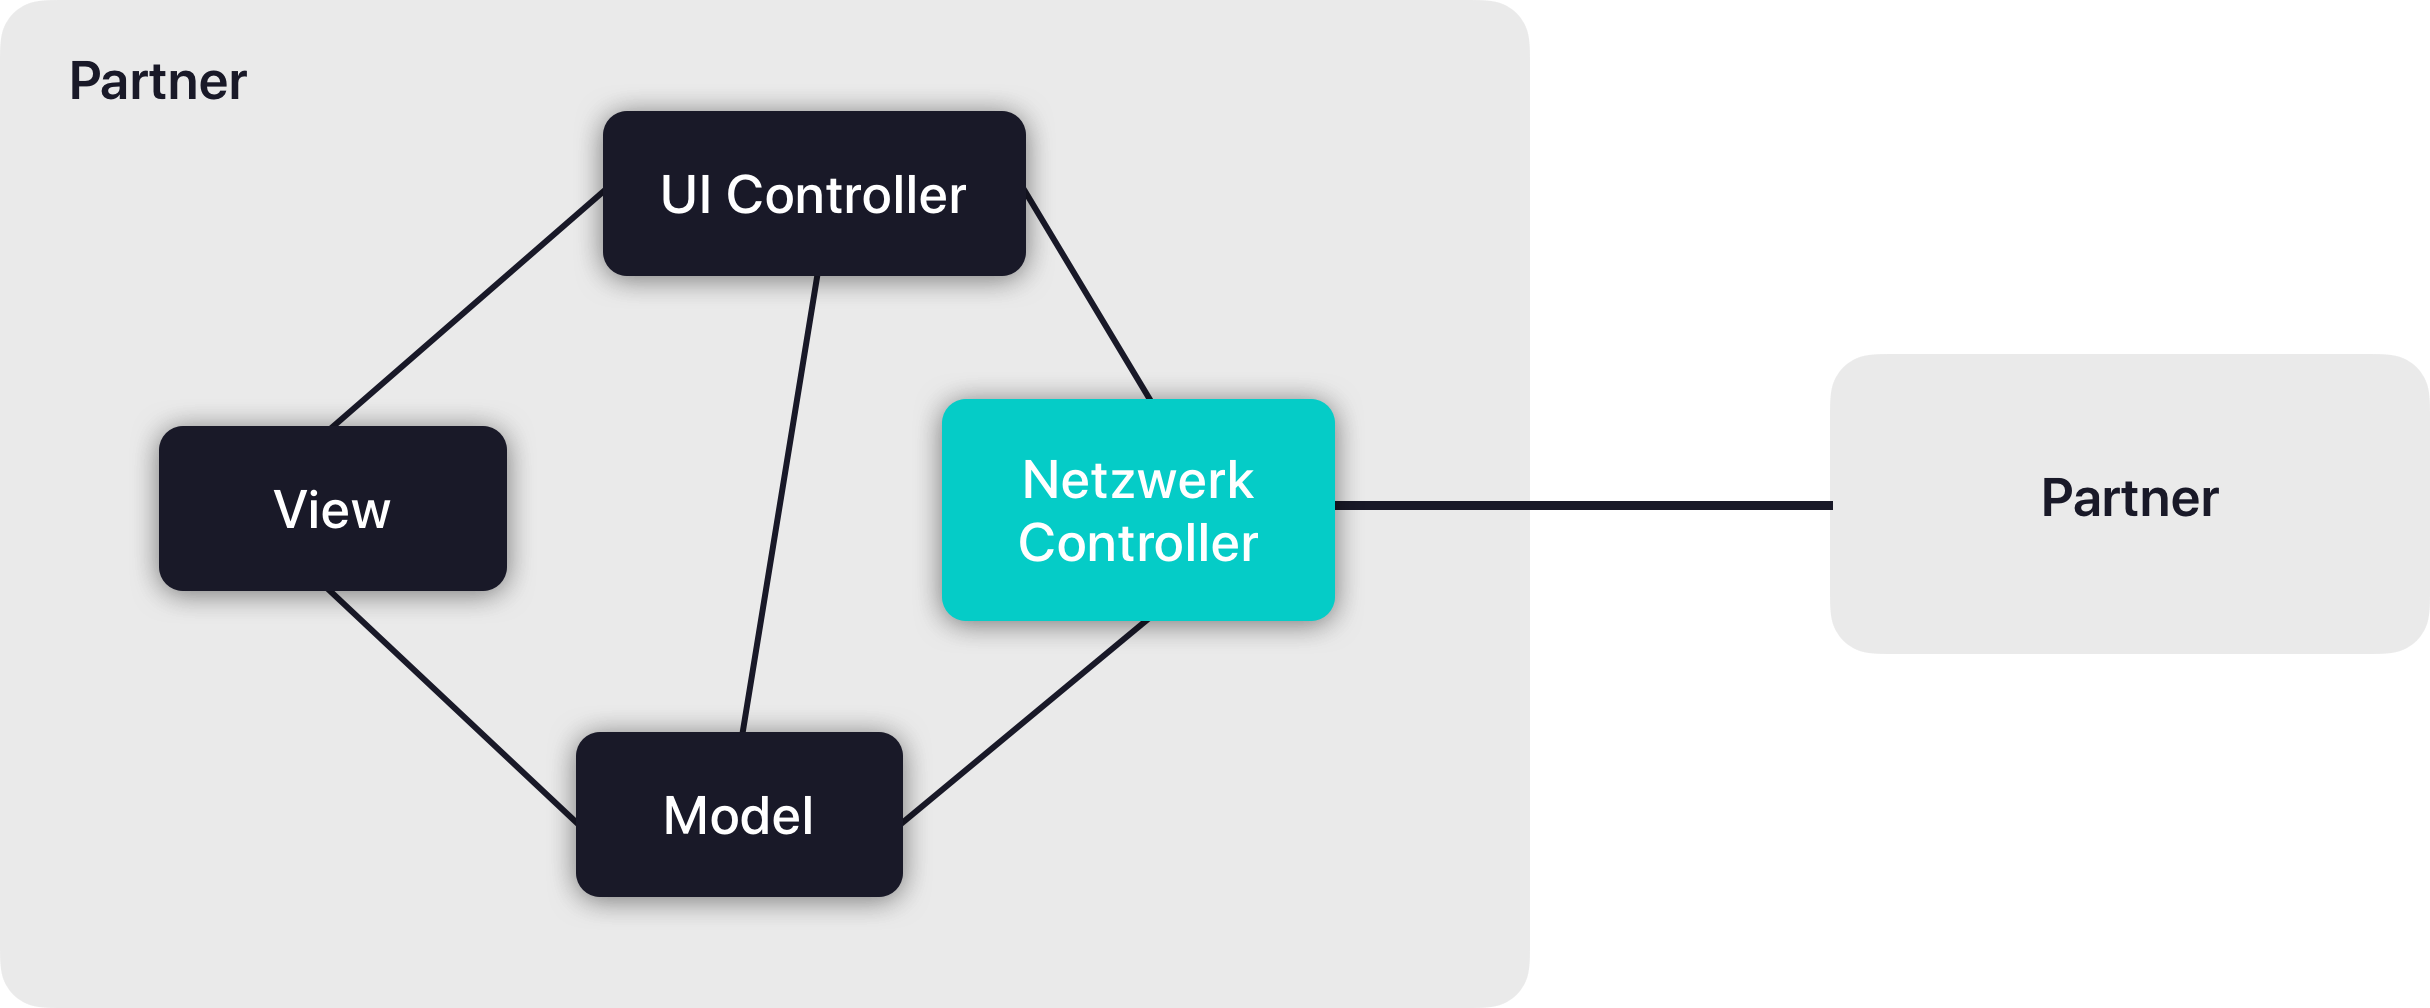
\includegraphics[width=1\textwidth]{graphics/Systemarchitektur}
  \caption{Schema der Systemarchitektur}
\end{figure}
Die Softwarearchitektur lässt sich auf zwei Ebenen betrachten, das Gesamtsystem mit der mobilen Anwendung des Patienten und der Desktopanwendung des Arztes oder einer weiteren mobilen Anwendung und die Teilsysteme auf den jeweiligen Geräten. \\\\
Da die einzelnen Geräte im Gesamtsystem gleichberechtigt miteinander kommunizieren sollen, wird es als Partnernetz realisiert.\\\\
Die Teilsysteme auf den Nutzergeräten enthalten lokale Daten, die in einer graphischen Benutzeroberfläche dargestellt werden sollen. Um die Datenverwaltung von der Darstellung zu trennen, wird die Model-View-Controller Architektur verwendet.

\section{Szenarien}
\subsection{Szenario: Patient lädt sich neue Daten auf myMD}
Greg ist ein neuer \gls{Nutzer} von myMD. Deshalb hat er auf seinem Konto auch noch keine \glspl{Arztbrief} eingetragen. Also geht er zu seinem Hausarzt, um seine Krankenakte für die myMD \gls{App} zu erhalten. Der Arzt öffnet dafür seine Praxissoftware und exportiert alle \glspl{Arztbrief}, die zu Greg gehören, und lädt diese in die \gls{Desktop Anwendung} von myMD. Sobald die \glspl{Arztbrief} im Sendetool angezeigt werden, klickt der Arzt auf den Button "Daten senden". Nun erhält Greg in seiner myMD \gls{App} eine Meldung und klickt "Daten empfangen". Auf Gregs myMD \gls{App} erscheint jetzt die Nachricht, dass die Daten an ihn gesendet werden. Sobald der Sendeprozess beendet ist, kann der Arzt die \gls{Desktop Anwendung} von myMD schließen und sich dem nächsten Patienten widmen. Greg hat jetzt all seine \glspl{Arztbrief} auf seinem Mobilgerät und kann sich diese jederzeit in der myMD \gls{App} anzeigen lassen. Sie werden im \gls{Tab} \textit{Übersicht} chronologisch sortiert dargestellt. Wenn er genauere Informationen zu einem bestimmten \gls{Arztbrief} einsehen möchte, kann er auf den \gls{Arztbrief} klicken und dieser wird nun auf dem ganzen Bildschirm, mit allen Informationen, dargestellt. So hat Greg jederzeit eine Übersicht.

\subsection{Szenario: Eigene Daten ansehen und editieren}
Greg leidet seit einigen Tagen unter starken Magenbeschwerden. Sein Hausarzt findet keine Ursache für die Beschwerden und überweist ihn deshalb an den Spezialisten Dr. Haus und verschreibt ihm etwas gegen die Schmerzen. Dr. Haus glaubt die Ursache gefunden zu haben, diese lässt sich aber nur durch eine Operation beseitigen, für die er Greg an einen Chirurgen überweist. \\
Bevor er dem Eingriff zustimmt, will er sich noch eine zweite Meinung einholen. Dafür lässt er sich von seinem Hausarzt einen weiteren Spezialisten empfehlen, der jedoch keine medizinische Ursache für das Problem erkennen kann. Er empfiehlt Greg eine psychotherapeutische Behandlung und verschreibt ihm zur Überbrückung ein stärkeres Schmerzmittel. \\ 
Bei so vielen verschiedenen Ärzten und Diagnosen hat Greg nun etwas den Überblick verloren. Glücklicherweise hat er bei seinen Arztbesuchen myMD verwendet und hat nun alle relevanten Daten auf seinem Mobilgerät gesammelt und kann sich in der App einen Überblick verschaffen. Letztendlich entscheidet sich Greg, es mit der Psychotherapie zu versuchen und entfernt die nun überflüssigen, schwächeren Schmerzmittel aus der Liste seiner Medikationen in myMD. 

\subsection{Szenario: Patient gibt behandelndem Arzt Daten zur Einsicht frei}
Gregs Beschwerden wollen kein Ende nehmen. Um der Ursache auf die Schliche zu kommen, überweist ihn sein Hausarzt nun an einen Gastroenterologen. Wie üblich bei neuen Patienten, möchte sich dieser zunächst mittels einer \gls{Anamnese} einen Überblick über den Stand der Dinge verschaffen. Dank der myMD \gls{App} hat Greg jederzeit all seine \glspl{Arztbrief} bei sich und kann diese nun seinem behandelnden Arzt zur Einsicht freigeben. Hierfür navigiert Greg in der myMD App in den \gls{Tab} \textit{Senden}, wo er nun aus einer Liste all seiner \glspl{Arztbrief} jene auswählen kann, die er mit seinem Arzt teilen möchte. Greg entschließt sich dazu, nur \glspl{Arztbrief} der letzten 6 Monate zu übertragen. \\
Per Knopfdruck beginnt das verschlüsselte Senden der Daten per \gls{Bluetooth} an den Computer des Arztes, auf welchem der Desktop-Klient von myMD die Daten verarbeitet und dem Arzt präsentiert. Schnell vermutet dieser, dass eine Wechselwirkung zwischen zwei eingenommenen \gls{Medikament}en die wahrscheinlichste Ursache für Gregs Leiden ist.

\section{Anwendungsfälle}
\subsection{Datenübertragung}
\begin{figure}[H]
\centering
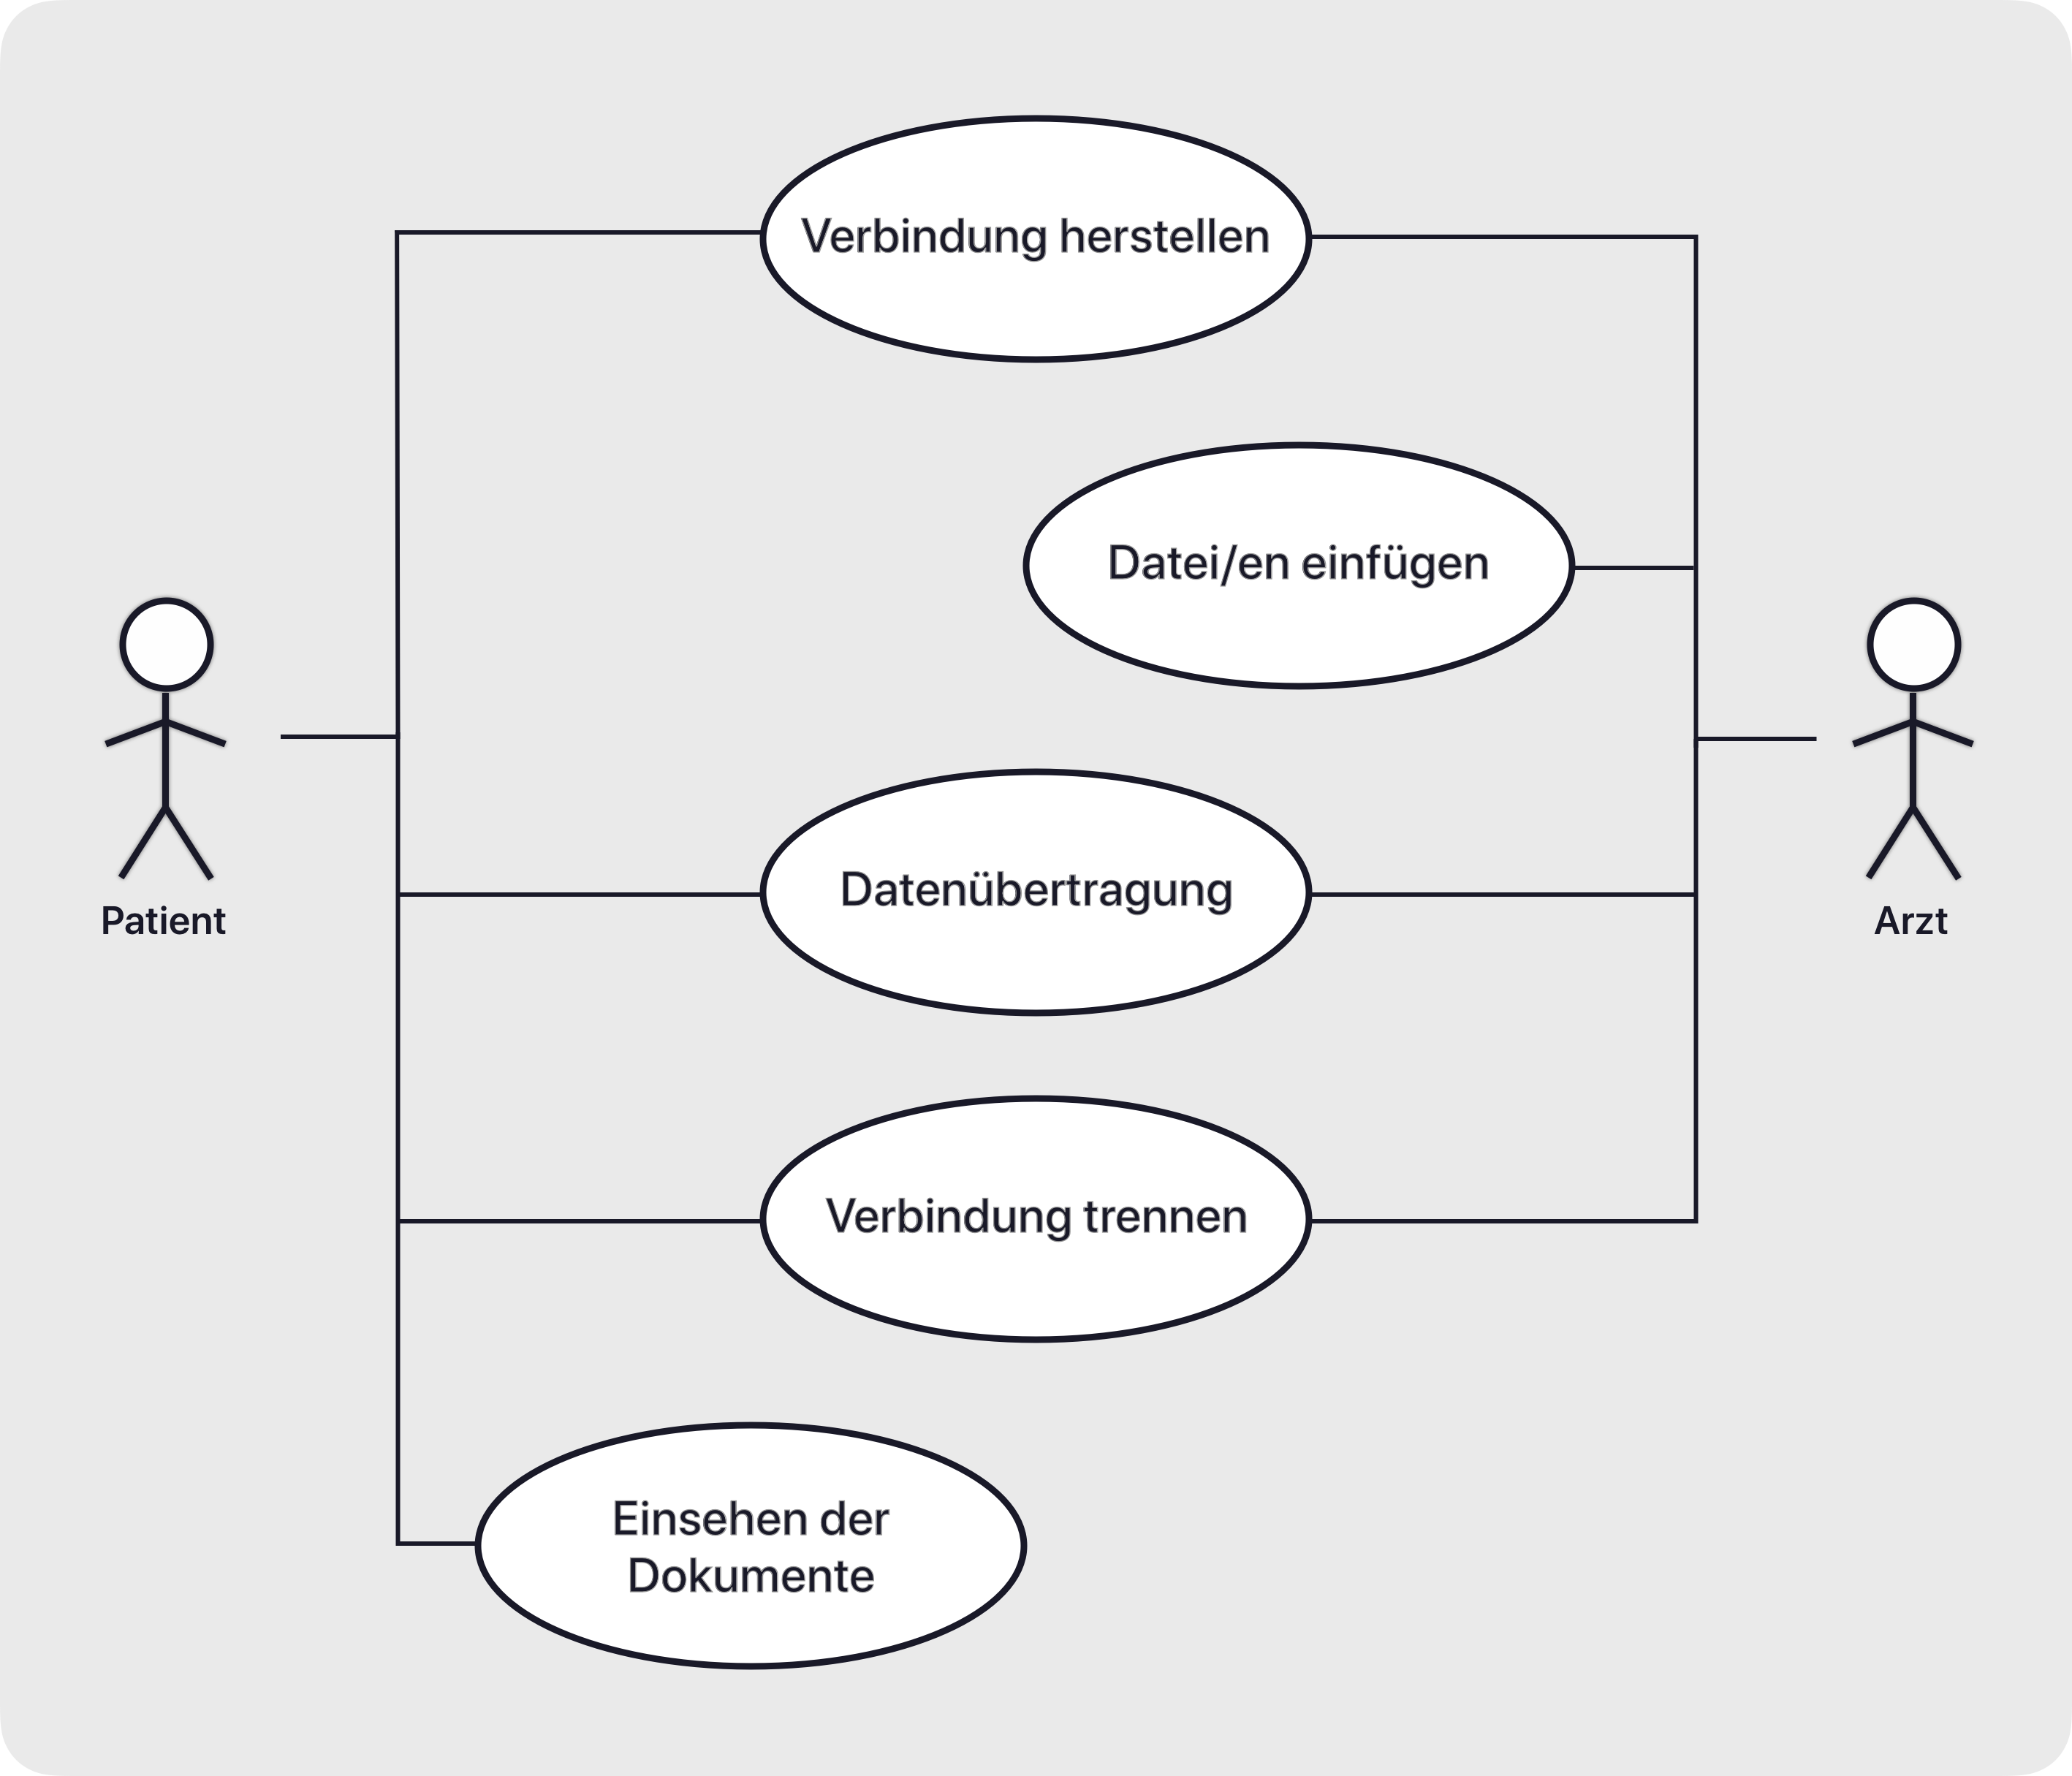
\includegraphics[width=0.8\textwidth]{graphics/AF-ArztPatient}
\caption{Anwendungsfall Datenübertragung Arzt-Patient}
\end{figure}

\begin{tabular}{lll}
{\textbf{Name}} & \multicolumn{2}{p{11.5cm}}  {Datenübertragung Arzt-Patient}\\
{\textbf{Teilnehmende Akteure}} & \multicolumn{2}{p{11.5cm}} {Patient, Arzt} \\
{\textbf{Eingangsbedingung}} & \multicolumn{2}{p{11.5cm}} {Der Patient hat die myMD \gls{App}, der Arzt die \gls{Desktop Anwendung} installiert} \\
{\textbf{Ausgangsbedingung}} & \multicolumn{2}{p{11.5cm}} {Die Daten wurden erfolgreich übertragen oder der Vorgang wird abgebrochen} \\
{\textbf{Ereignisfluss}} & \multicolumn{2}{p{11.5cm}} {Verbindung zwischen Arzt und Patienten wird hergestellt $\Rightarrow$ Arzt fügt zu übertragende Daten in die Anwendung ein $\Rightarrow$ Die Daten werden vom Arzt zum Patienten übertragen $\Rightarrow$ Verbindung zwischen Arzt und Patient wird getrennt $\Rightarrow$ Patient kann Daten einsehen} \\
{\textbf{Spezielle Anforderungen}} & \multicolumn{2}{p{11.5cm}} {Drahtlosverbindung zwischen Arzt und Patient} \\
\end{tabular} 

\subsection{Nutzerprofil}
\begin{figure}[H]
\centering
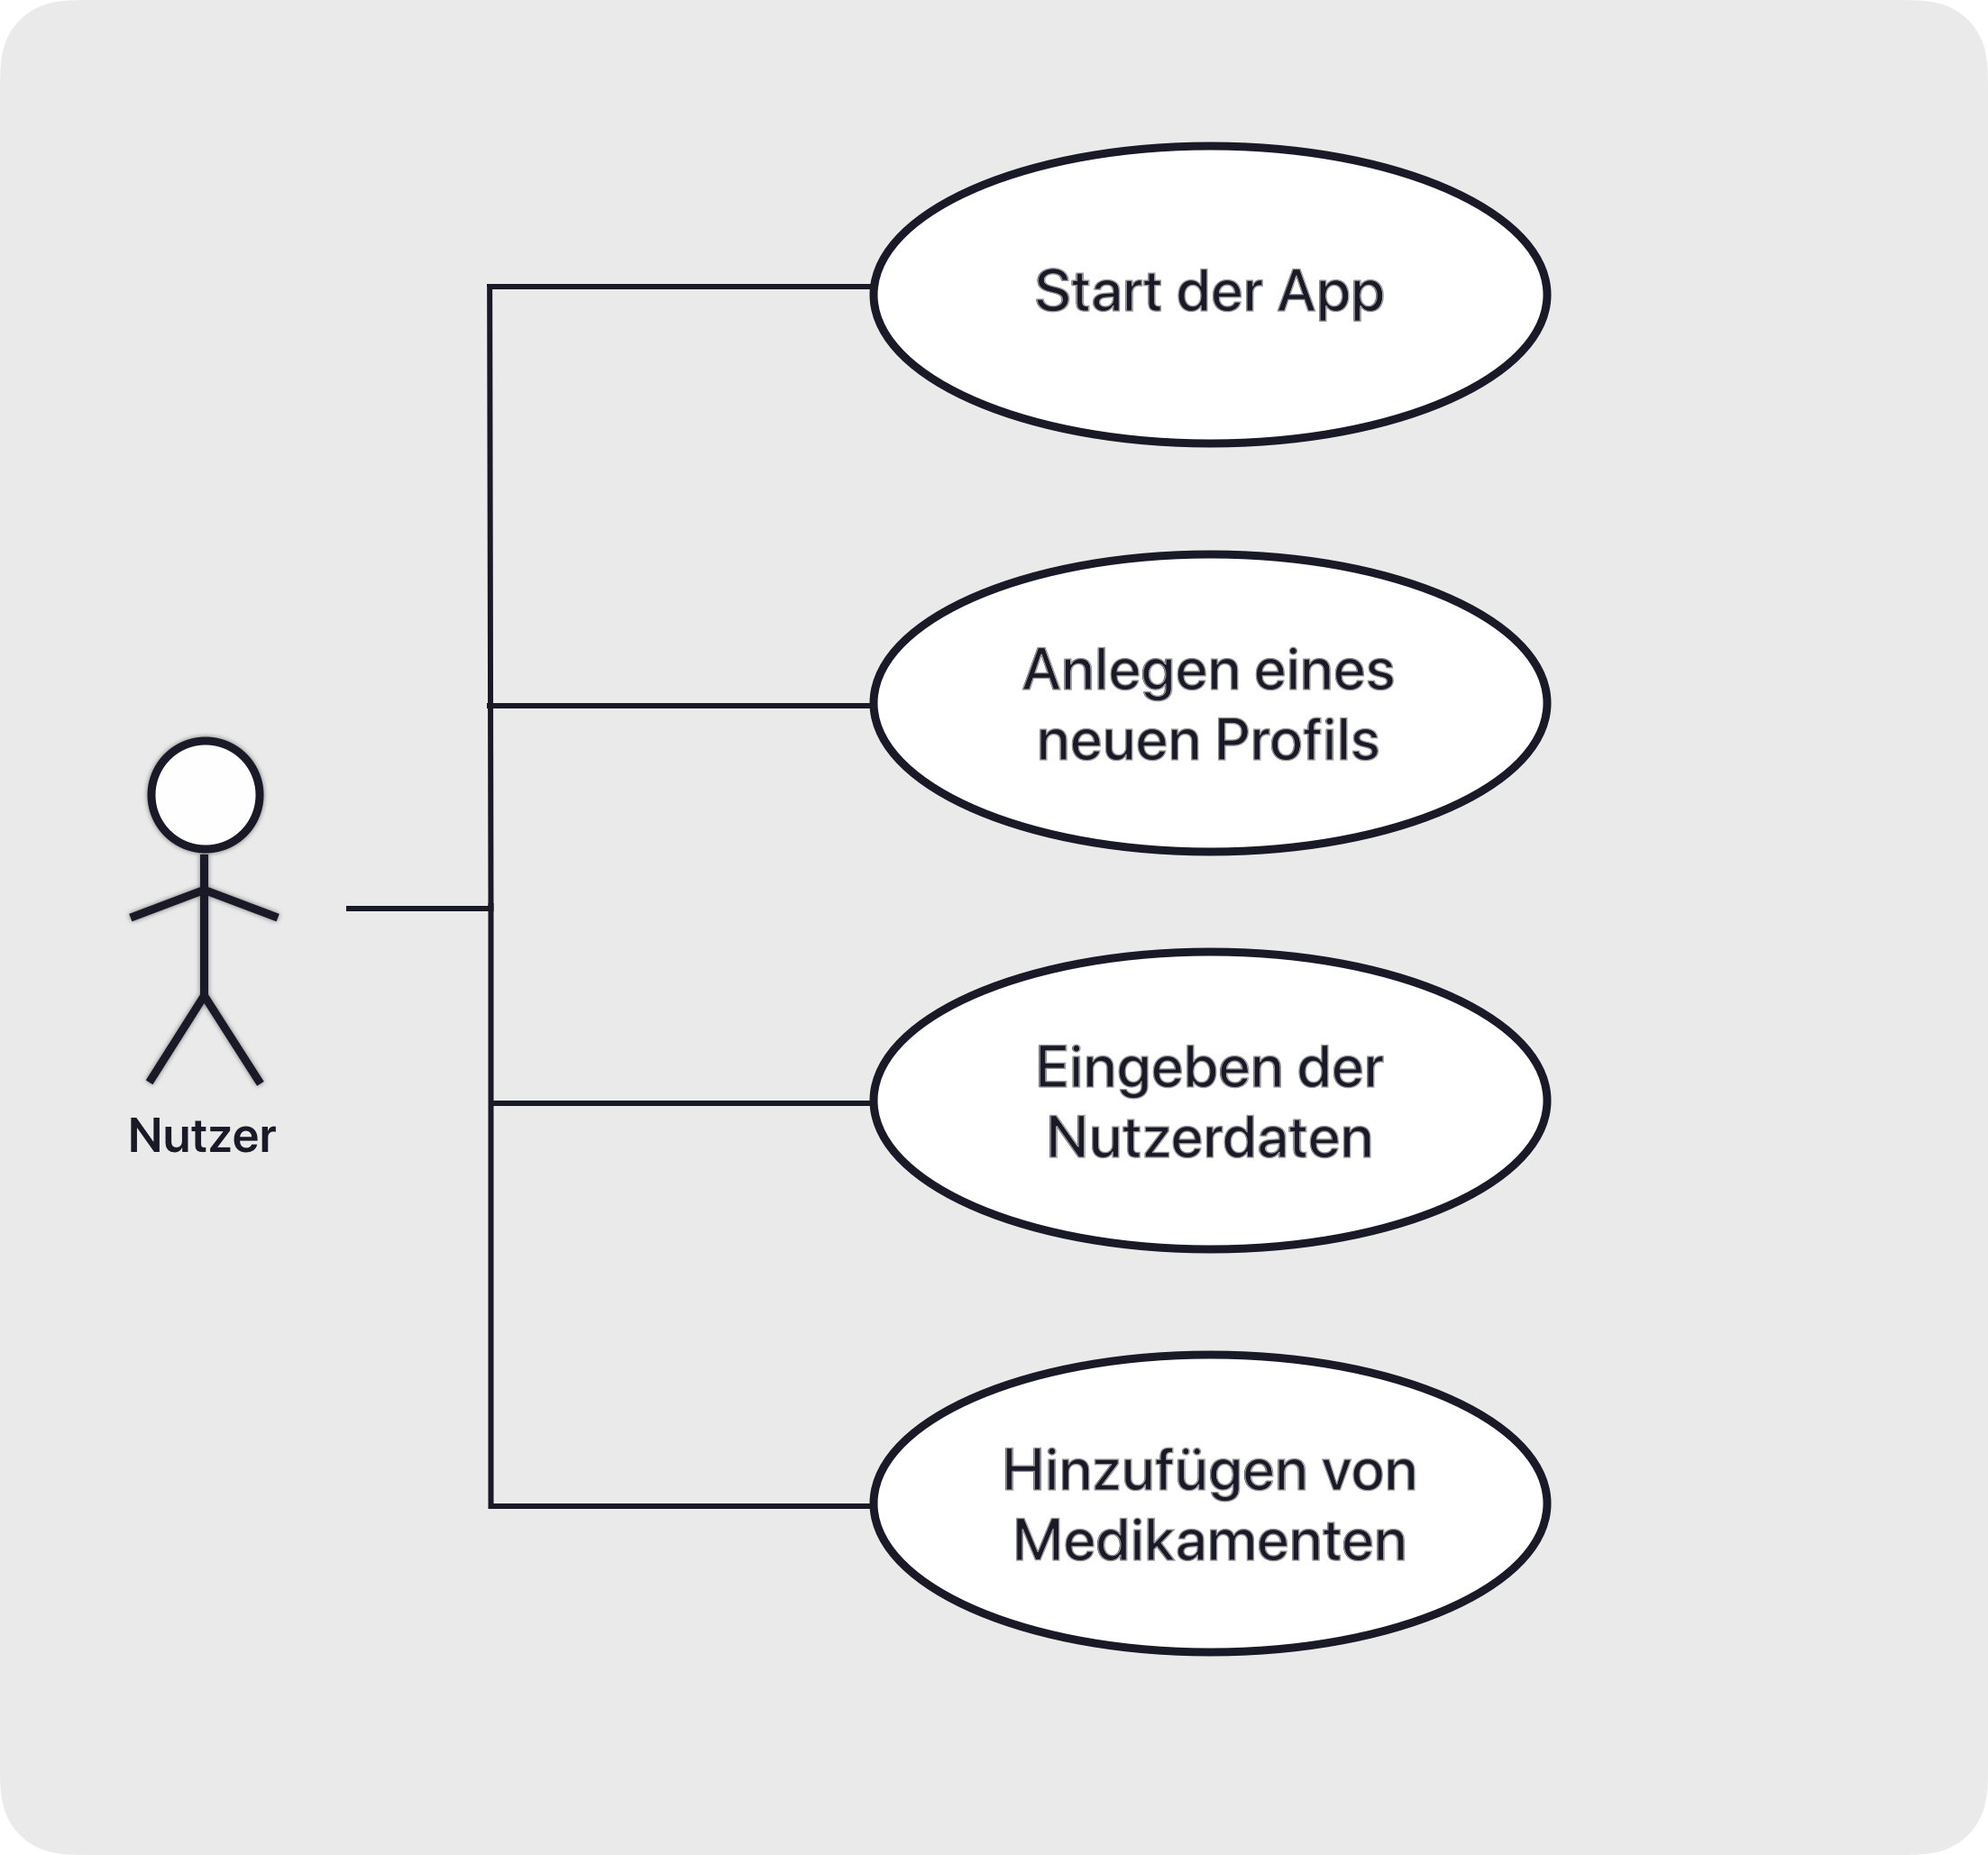
\includegraphics[width=0.8\textwidth]{graphics/AF-NeuerNutzer}
\caption{Anwendungsfall Neuer \gls{Nutzer}}
\end{figure}

\begin{tabular}{lll}
{\textbf{Name}} & \multicolumn{2}{p{11.5cm}} {Neuer \gls{Nutzer}}\\
{\textbf{Teilnehmende Akteure}} & \multicolumn{2}{p{11.5cm}} {\gls{Nutzer}} \\
{\textbf{Eingangsbedingung}} & \multicolumn{2}{p{11.5cm}} {Der \gls{Nutzer} hat die myMD \gls{App} installiert} \\
{\textbf{Ausgangsbedingung}} & \multicolumn{2}{p{11.5cm}} {Der \gls{Nutzer} hat alle gewünschten Daten eingegeben oder den Vorgang abgebrochen} \\
{\textbf{Ereignisfluss}} & \multicolumn{2}{p{11.5cm}} {Ereignisfluss: \gls{Nutzer} startet App $\Rightarrow$ Neues Profil erstellen $\Rightarrow$ \gls{Nutzer}-Informationen eingeben $\Rightarrow$  \gls{Medikament}e hinzufügen} \\
{\textbf{Spezielle Anforderungen}} & \multicolumn{2}{p{11.5cm}} {Keine} \\
\end{tabular} 

\begin{figure}
\section{Benutzeroberfläche}


\captionsetup{singlelinecheck=false, justification = justified}
\begin{minipage}[t][][b]{0.4\textwidth}
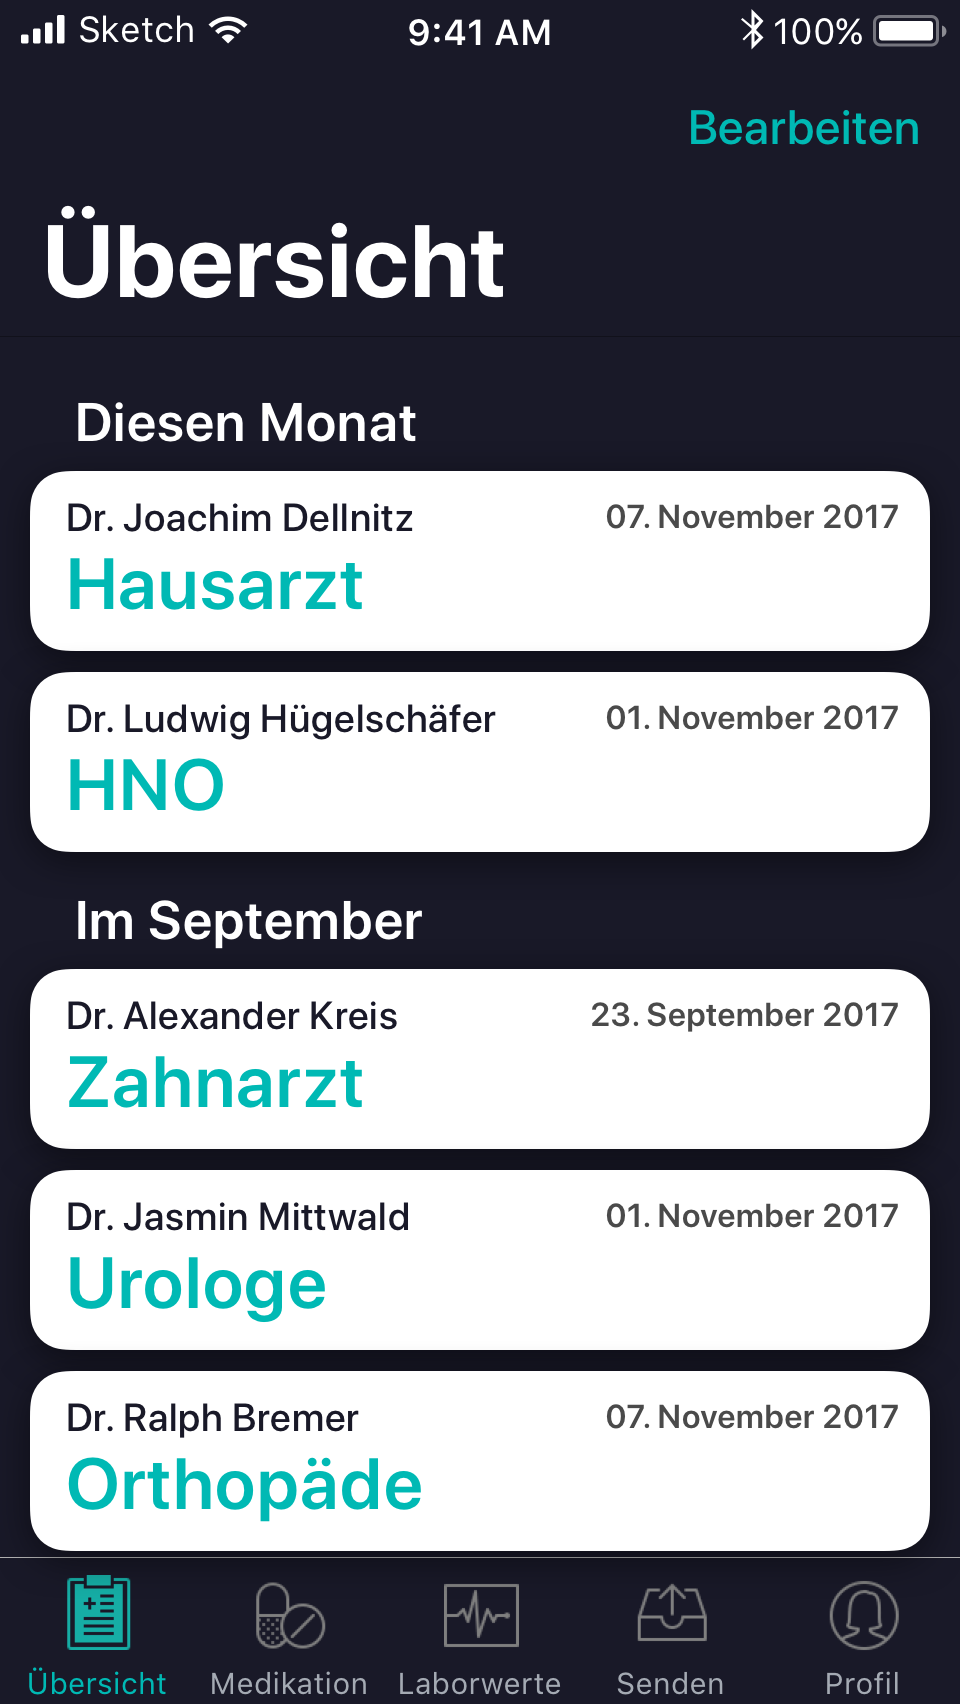
\includegraphics[width=0.9\textwidth]{mockups/OverviewTab}
\captionof{figure}{\gls{Tab} \textit{Übersicht}}
~\\
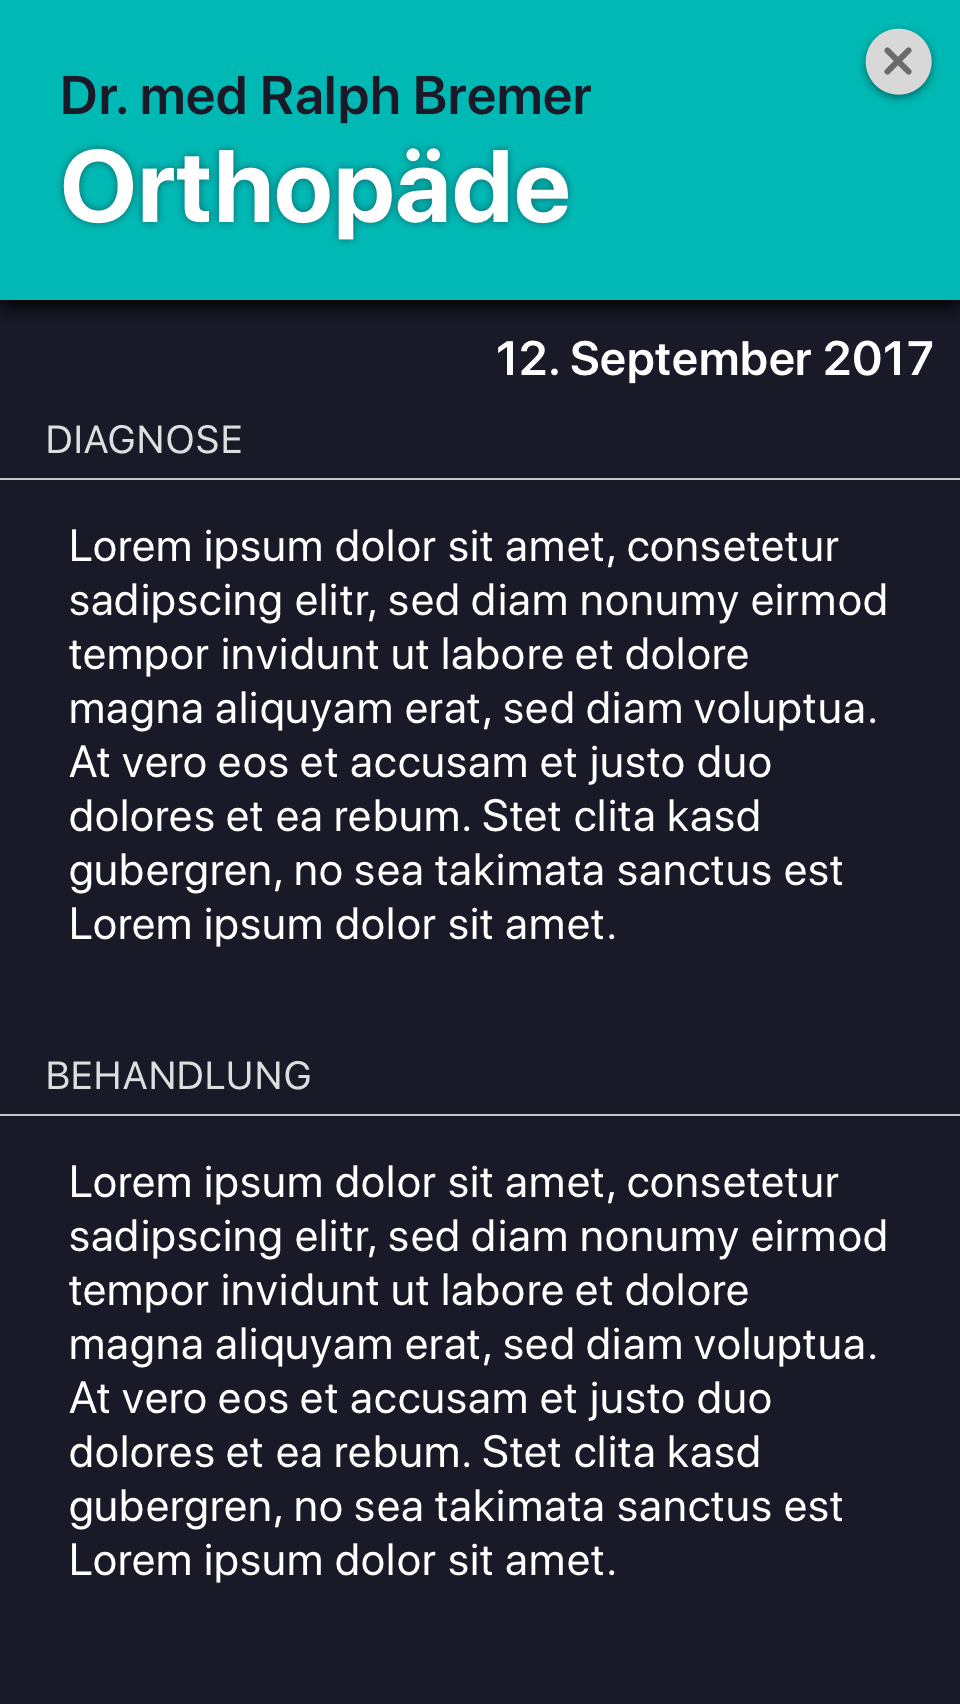
\includegraphics[width=0.9\textwidth]{mockups/ArztbriefDetailed}
\captionof{figure}{\gls{Arztbrief} in detaillierter Ansicht}
\end{minipage}%
\hfill
\begin{minipage}[t][][b]{0.65\textwidth}

\subsection*{Tab \textit{Übersicht}}
\textbf{Beschreibung}\\
{Darstellung der Übersicht über alle verfügbaren \glspl{Arztbrief}}\\
~\\
\textbf{Elemente}\\
{\glspl{Arztbrief} als Listenelemente}\\
{Button: Löschen von Einträgen}\\
{Tab Bar: Navigieren durch die App}\\

\textbf{Verwendung}\\
{Tippen auf einen Listeneintrag öffnet eine detaillierte Vollbild-Ansicht zu diesem Eintrag.}\\
{Durch vertikales Wischen kann durch die Auflistung aller \glspl{Arztbrief} navigiert werde.n}\\
{Horizontales Wischen vom rechten Rand eines Listenelements nach links löscht den Eintrag.}\\
\newline
\newline
\newline

\subsection*{Detaillierter \gls{Arztbrief}}
\textbf{Beschreibung}\\
{Vollständige Darstellung eines Arztbriefes}\\
~\\
\textbf{Elemente}\\
{Textbox: Name des Arztes}\\
{Textbox: Fachrichtung des Arztes}\\
{Textbox: Erstellungsdatum des Arztbriefes}\\
{Textbox: Ausgestellte Diagnose}\\
{Textbox: Behandlungsbeschreibung}\\

\textbf{Verwendung}\\
{In dieser Ansicht können Diagnose und Behandlung eines Arztbesuches näher studiert werden. }\\
{Dazu kann durch vertikales Wischen durch die Texte gescrollt werden.}
\end{minipage}%
\end{figure}

\newpage

\begin{minipage}[t][][b]{0.4\textwidth}

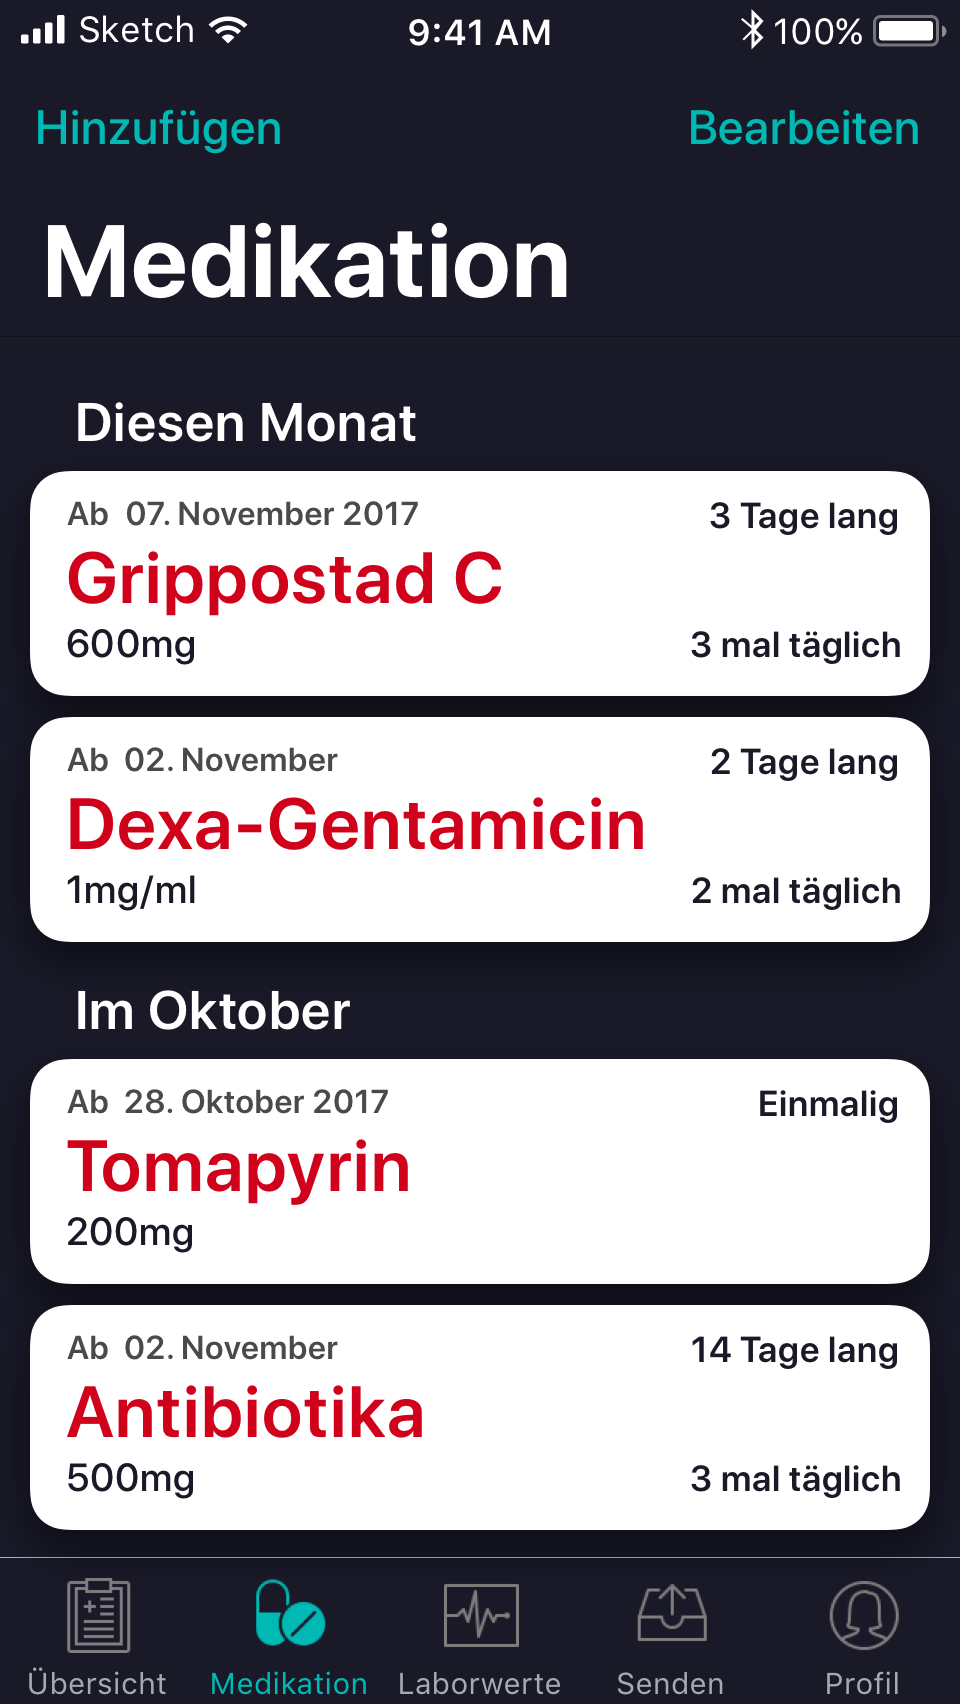
\includegraphics[width=0.9\textwidth]{mockups/MedTab}
\captionof{figure}{\gls{Tab} \textit{Medikation}}
~\\
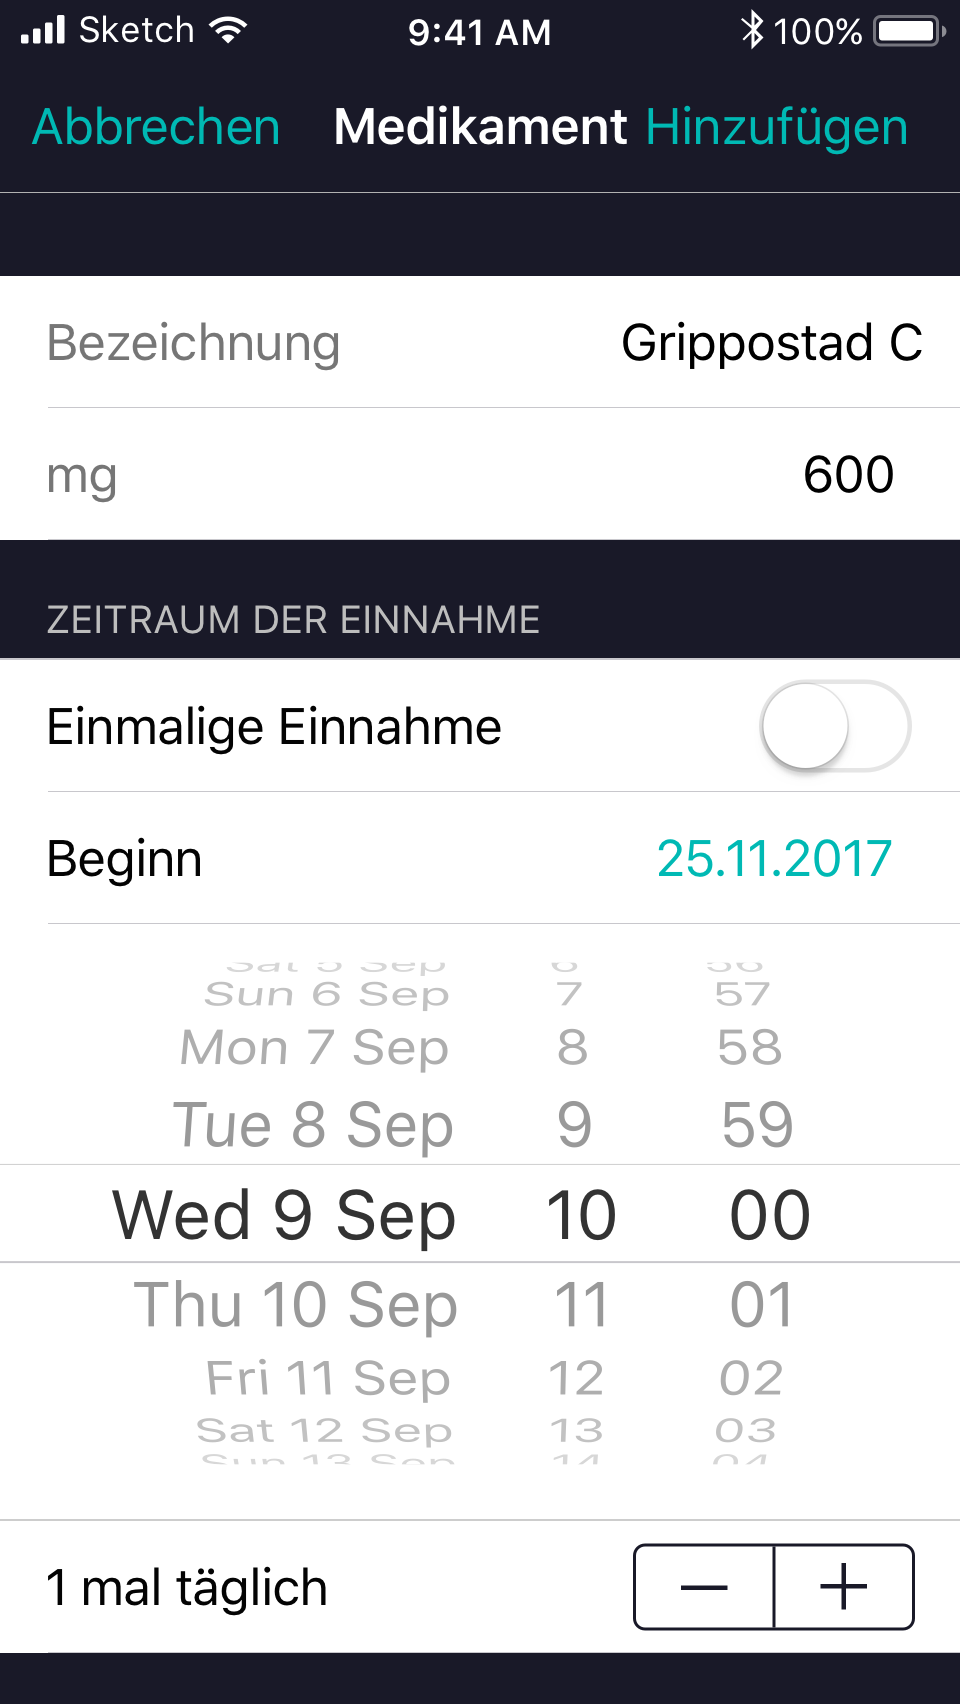
\includegraphics[width=0.9\textwidth]{mockups/NewMed}
\captionof{figure}{Ansicht beim Hinzufügen\\ eines \gls{Medikament}s}

\end{minipage}%
\hfill
\begin{minipage}[t][][b]{0.65\textwidth}
\subsection*{Tab \textit{Medikation}}
\textbf{Beschreibung}\\
{Auflistung aller eingepflegter \gls{Medikament}eneinnahmen}\\
~\\
\textbf{Elemente}\\
{Eingenommene \gls{Medikament}e als Listenelemente}\\
{Button: Bearbeiten von Einträgen}\\
{Button: Hinzufügen eines \gls{Medikament}es}\\
{Textfelder: Details einer \gls{Medikament}eneinnahme}\\

\textbf{Verwendung}\\
{Durch vertikales Wischen kann durch die Auflistung aller eingenommener \gls{Medikament}e navigiert werden.}\\
{Horizontales Wischen vom rechten Rand eines Listenelements nach links löscht den Eintrag.}\\
{Tippen auf \textit{Hinzufügen} öffnet ein Formular zum Einpflegen eines neuen \gls{Medikament}es.}

\subsection*{Neue \gls{Medikament}eneinnahme hinzufügen}
\textbf{Beschreibung}\\
{Formular zum Festlegen von \gls{Medikament}enparameter}\\
~\\
\textbf{Elemente}\\
{Button: Abbrechen des Vorgangs}\\
{Button zum Abschließen des Vorgangs}\\
{Textbox: Bezeichnung des \gls{Medikament}es}\\
{Textbox: Dosierung des Wirkstoffes}\\
{Schalter: Einmalig einzunehmendes \gls{Medikament}?}\\
{Button: Festlegen des Einnahmebeginns}\\
{Button: Festlegen der Einnahmehäufigkeit}\\

\textbf{Verwendung}\\
{In dieser Ansicht können die Details zu einem neuen \gls{Medikament} eingetragen werden oder Angaben zu einem bereits angelegten \gls{Medikament} korrigiert werden.}
\end{minipage}%


\newpage


\begin{minipage}[t][][b]{0.4\textwidth}

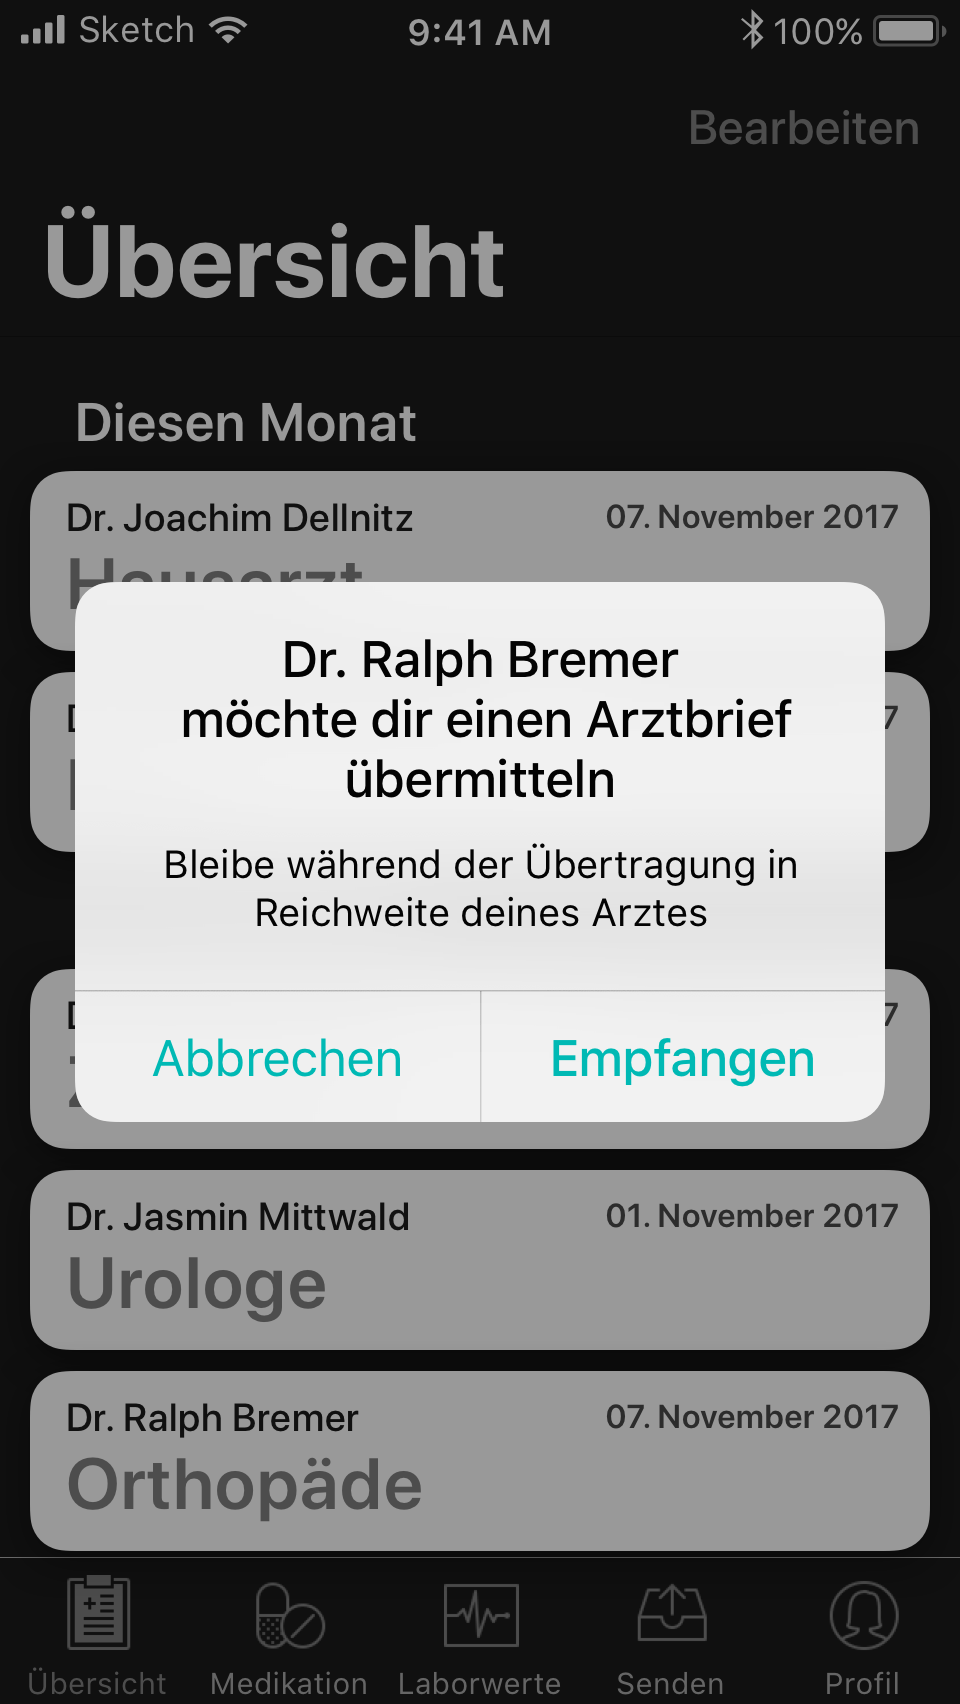
\includegraphics[width=0.9\textwidth]{mockups/ReceiveData}
\captionof{figure}{Übertragungsanfrage des \\Arztes}
~\\
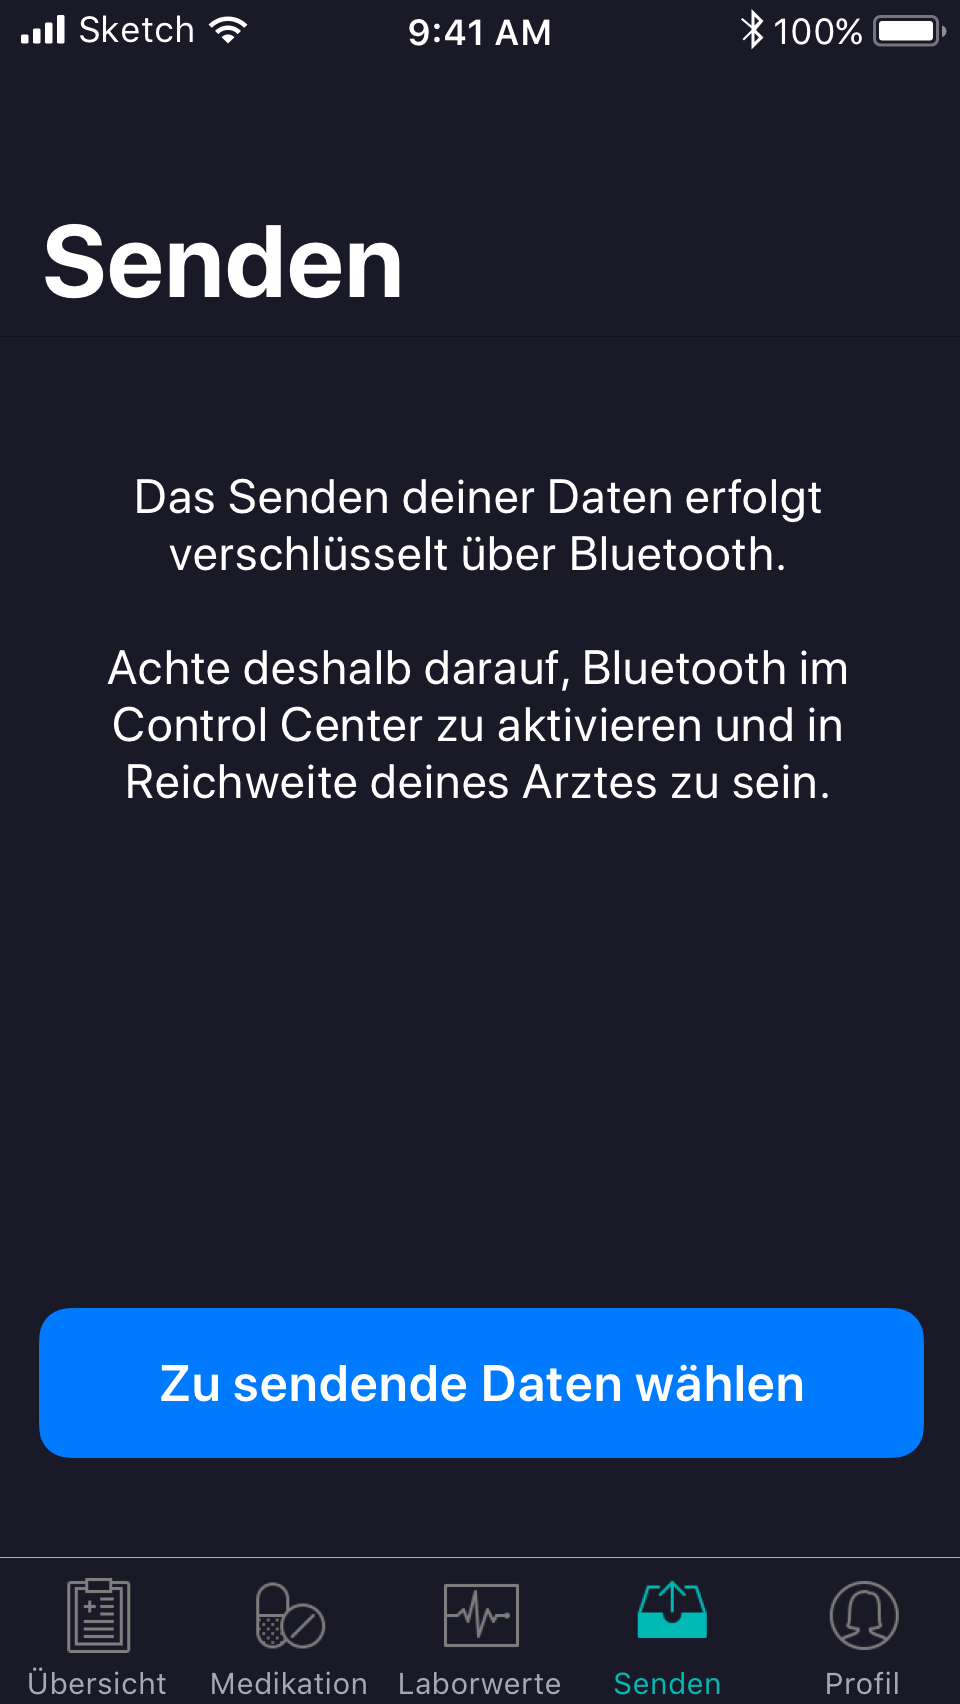
\includegraphics[width=0.9\textwidth]{mockups/SendTab}
\captionof{figure}{\gls{Tab} \textit{Senden}}
\end{minipage}%
\hfill
\begin{minipage}[t][][b]{0.65\textwidth}
\subsection*{Übermittlungsanfrage}
\textbf{Beschreibung}\\
{Meldung im Falle einer Übermittlungsanfrage des Arztes}\\
~\\
\textbf{Elemente}\\
{\gls{Pop-Up}: Nachricht mit Name des anfragenden Arztes}\\
{Button: Ablehnen der Anfrage}\\
{Button: Zustimmen der Anfrage}\\

\textbf{Verwendung}\\
{Hier kann der \gls{Nutzer} entscheiden, ob er einer Übertragungsanfrage des Arztes zustimmen oder sie ablehnen möchte.}

~\\
~\\
~\\

\subsection*{Senden von Arztbriefen}
\textbf{Beschreibung}\\
{Darstellung des Tabs \textit{Senden}}\\
~\\
\textbf{Elemente}\\
{Textbox: Nutzerhinweise zum Sendevorgang}\\
{Button: Starten des Auswahlvorgangs von Arztbriefen}\\
~\\
\textbf{Verwendung}\\
{Sollte sich der \gls{Nutzer} entschließen, \glspl{Arztbrief} an einen Arzt zu übermitteln, öffnet der große Knopf in der unteren Bildschirmhälfte eine Liste aller \glspl{Arztbrief} auf dem Gerät, aus denen der \gls{Nutzer} dann diejenigen auswählen kann, die er gerne versenden würde.}
\end{minipage}%



\newpage


\begin{minipage}[t][][b]{0.45\textwidth}

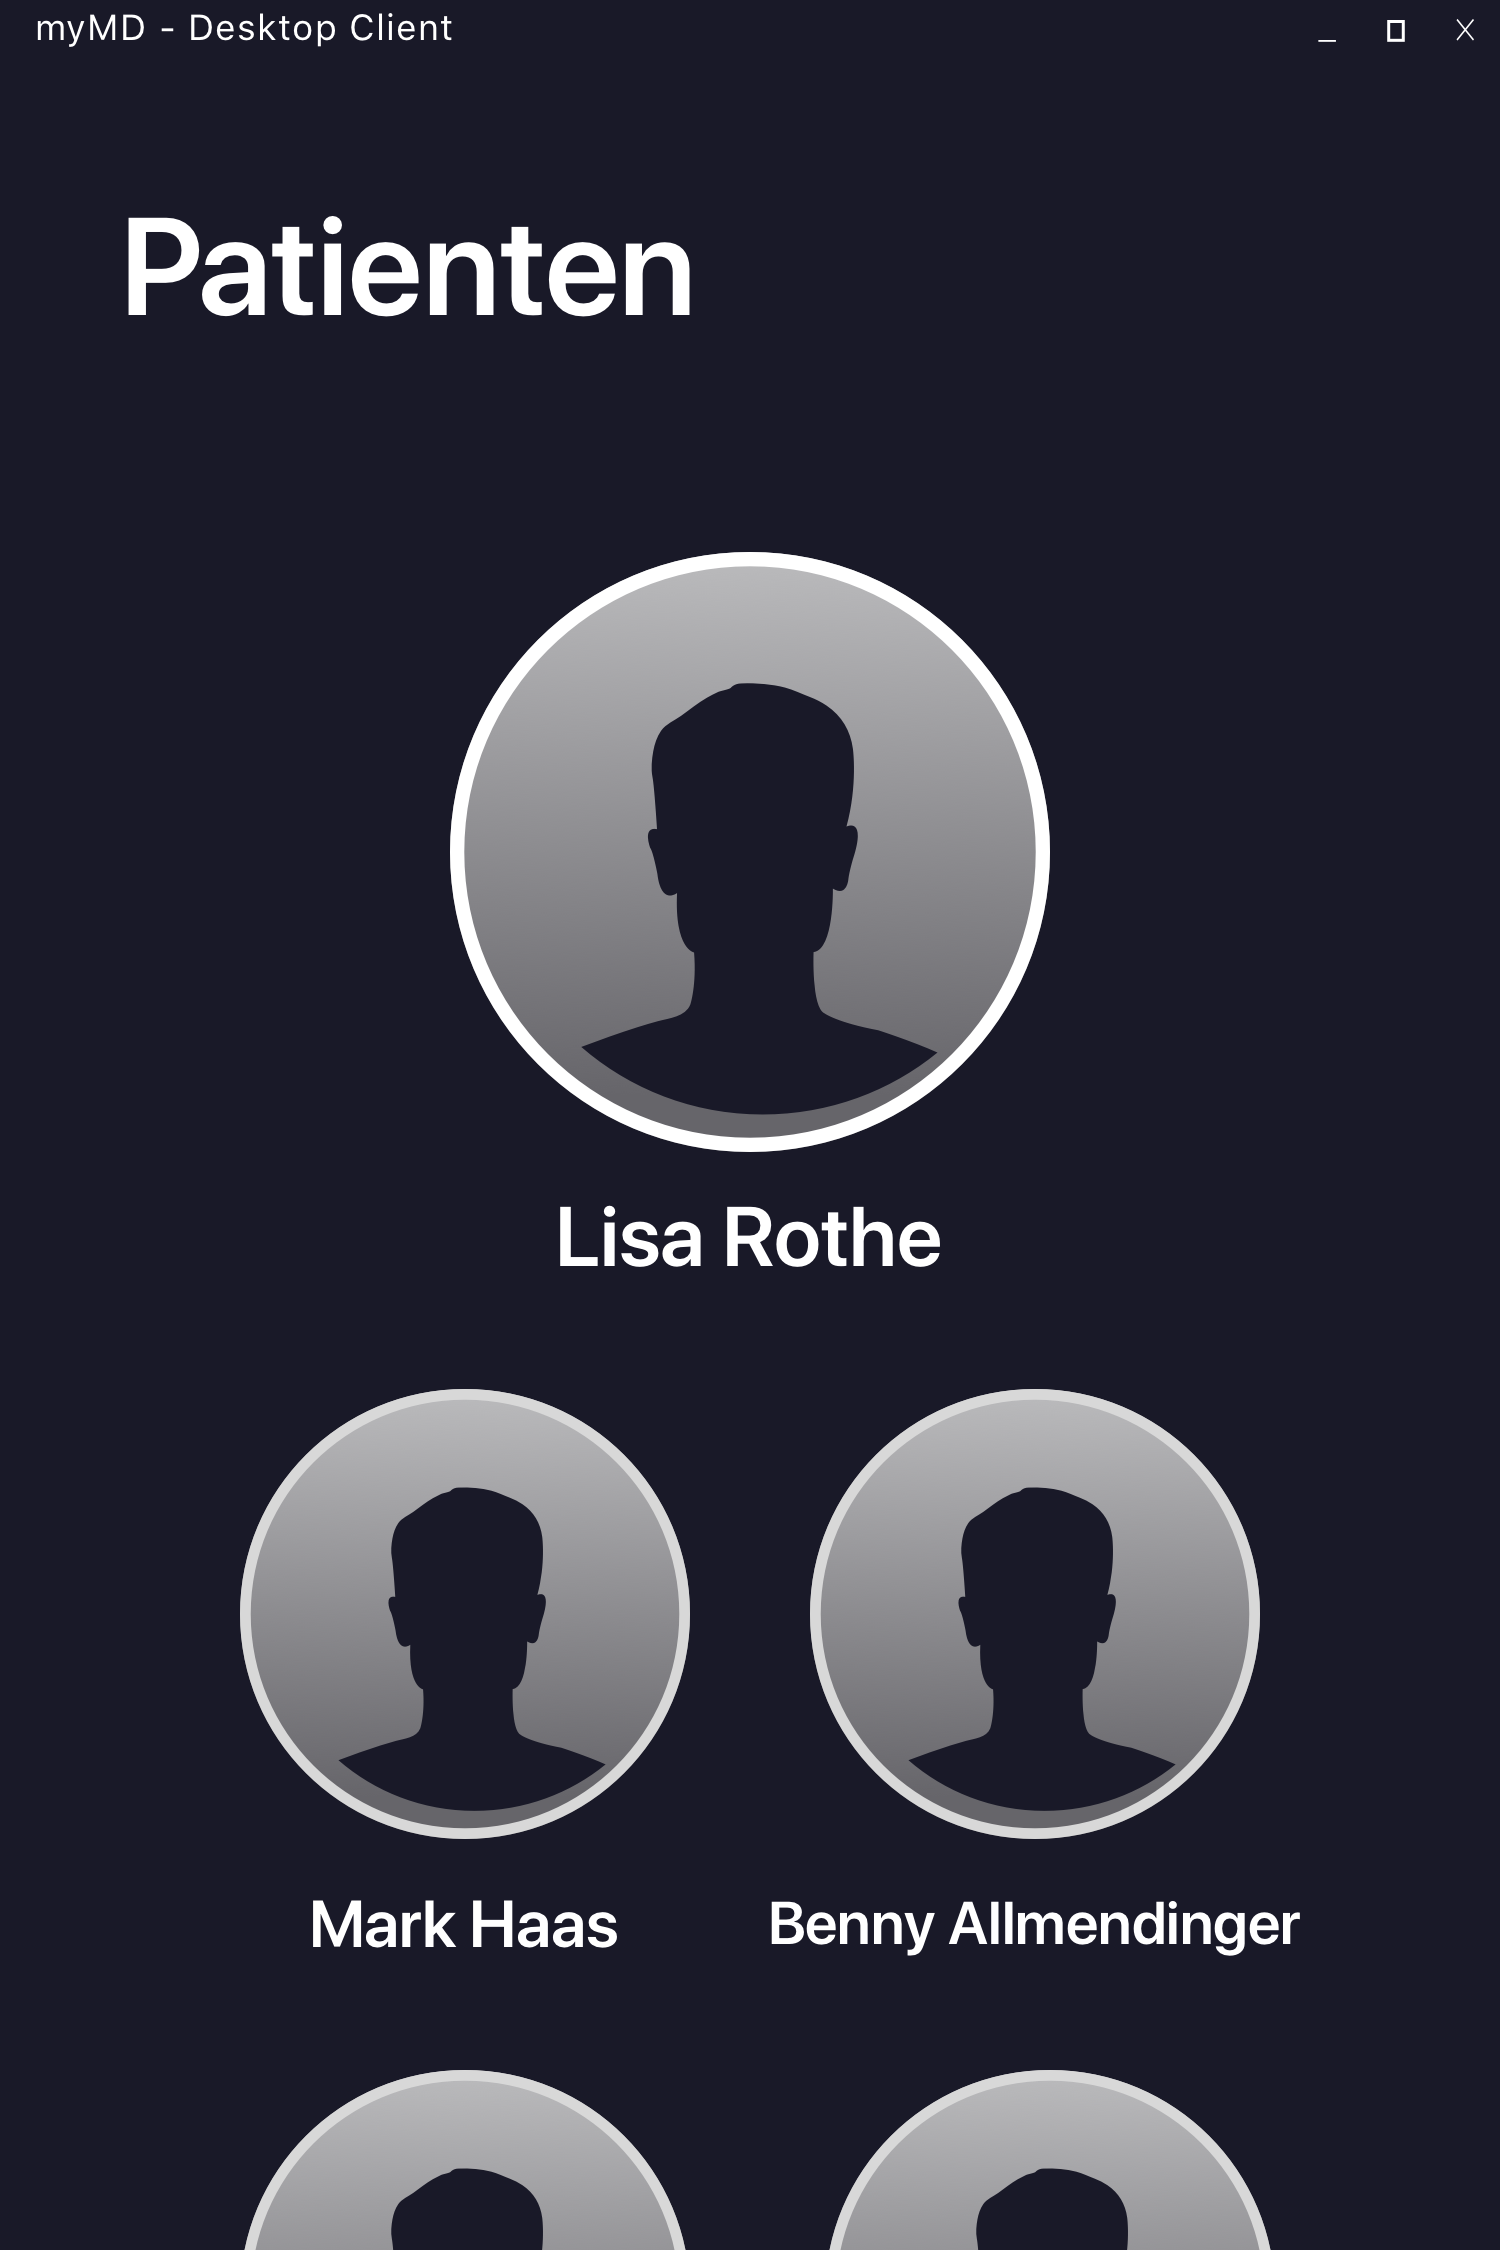
\includegraphics[width=0.9\textwidth]{mockups/SelectPatient}
\captionof{figure}{Auflistung aller Geräte \\in Reichweite}
~\\
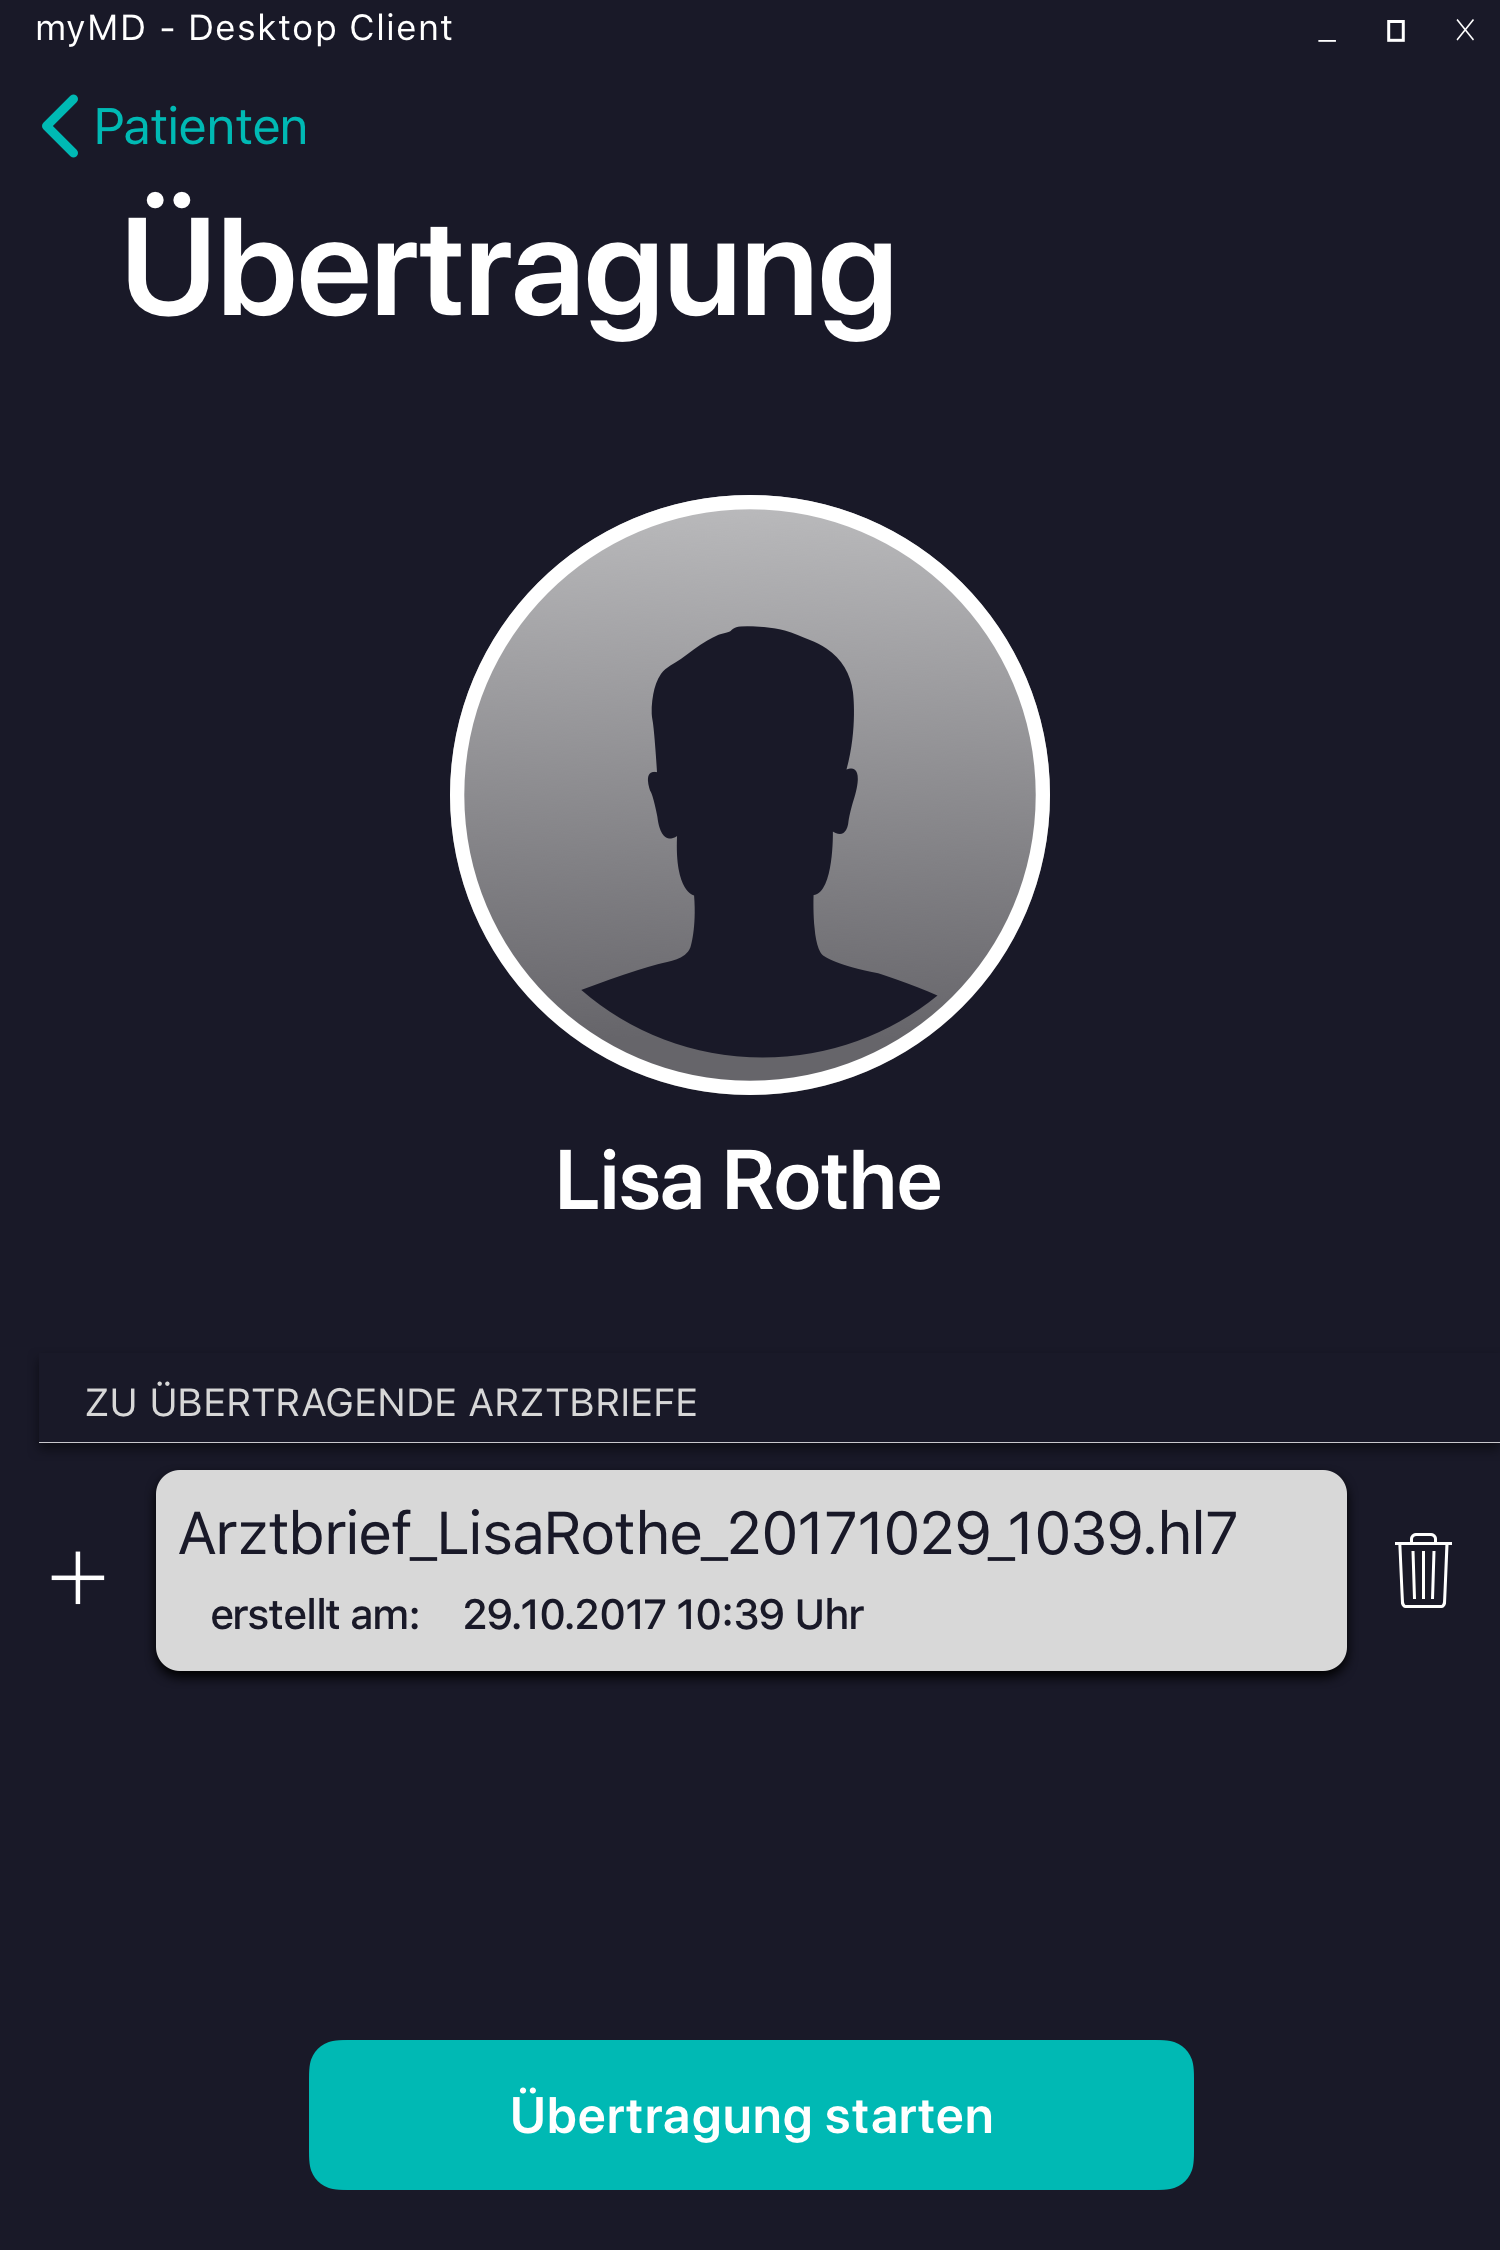
\includegraphics[width=0.9\textwidth]{mockups/SelectFiles}
\captionof{figure}{Importieren und Übertragen \\von Arztbriefen}
\end{minipage}%
\hfill
\begin{minipage}[t][][b]{0.55\textwidth}
\subsection*{Gerät eines Patienten suchen}
\textbf{Beschreibung}\\
{Ansicht der gefundenen Patientengeräte}\\
~\\
\textbf{Elemente}\\
{Kollektion: Alle Geräte in Reichweite}\\
{Buttons: Programm minimieren, maximieren \\oder schließen}\\

\textbf{Verwendung}\\
{Hier kann der Arzt alle Geräte sehen, die sich in Reichweite seines Computers befinden.}\\
{Sollte das gesuchte Gerät erscheinen, lässt es sich per Doppelklick auswählen, um Dateien übertragen zu können.}\\


\subsection*{\glspl{Arztbrief} an Patienten übertragen}
\textbf{Beschreibung}\\
{Fenster zur Auswahl und Übertragung der gewünschten \glspl{Arztbrief}}\\
~\\
\textbf{Elemente}\\
{Button: Zurück zur Geräte-Übersicht}\\
{Button: Hinzufügen einer Datei}\\
{Button: Löschen einer bereits hinzugefügten Datei}\\
{Button: Absenden der ausgewählten Dateien}\\
~\\
\textbf{Verwendung}\\
{Der Arzt hat nun die Möglichkeit, Dateien in die Anwendung zu importieren (\gls{Drag and Drop}, Datei-Explorer) und sie wieder zu entfernen. Hat er die gewünschten Dateien korrekt eingefügt, lassen sich diese über den Button am unteren Bildschirmrand zum Patienten übertragen.}
\end{minipage}%

\chapter{Testfälle}
\section{Basis Testfälle (BT)}

\subsection{Patientenseitige Datenübertragung}
\begin{tabular}{lll}
[BT1010] & \multicolumn{2}{p{12cm}}  {\gls{Desktop Anwendung} sendet eine Datei an die myMD \gls{App}.} \\
{[BT1020]} & \multicolumn{2}{p{12cm}}  {Die Übertragung wird vom \gls{Nutzer} unterbrochen.} \\
{[BT1030]} & \multicolumn{2}{p{12cm}}  {\gls{Desktop Anwendung} sendet eine unzulässige Datei (nicht unterstütztes Dateiformat).} \\
{[BT1040]} & \multicolumn{2}{p{12cm}}  {Die Übertragung wird durch äußere Umstände abgebrochen.} \\

\end{tabular}

\subsection{Darstellung}
\begin{tabular}{lll}
[BT2010] & \multicolumn{2}{p{12cm}}  {Ein neuer \gls{Arztbrief} wird in eine leere Übersicht geladen.} \\
{[BT2020]} & \multicolumn{2}{p{12cm}}  {Ein neuer \gls{Arztbrief} wird in bereits gefüllte Übersicht geladen.} \\
{[BT2030]} & \multicolumn{2}{p{12cm}}  {Ein digitaler \gls{Arztbrief} wird angetippt/geöffnet.} \\
{[BT2040]} & \multicolumn{2}{p{12cm}}  {Ein digitaler \gls{Arztbrief} wird geschlossen.} \\
{[BT2050]} & \multicolumn{2}{p{12cm}}  {Ein digitaler \gls{Arztbrief} wird gelöscht.} \\

\end{tabular}

\subsection{Einstellungen}
\begin{tabular}{lll}
{[BT3010]} & \multicolumn{2}{p{12cm}}  {Das Nutzerprofil wird bearbeitet.} \\
\end{tabular}

\subsection{\gls{Desktop Anwendung}}
\begin{tabular}{lll}
{[BT4010]} & \multicolumn{2}{p{12cm}}  {Unzulässige Datei wird zum Senden ausgewählt.} \\
{[BT4020]} & \multicolumn{2}{p{12cm}}  {Kompatible Datei wird zum Senden ausgewählt.} \\
{[BT4030]} & \multicolumn{2}{p{12cm}}  {Senden wird erfolgreich abgeschlossen.} \\
{[BT4040]} & \multicolumn{2}{p{12cm}}  {Senden wird durch äußere Einflüsse unterbrochen.} \\
{[BT4050]} & \multicolumn{2}{p{12cm}}  {Senden wird durch \gls{Nutzer} unterbrochen.} \\
{[BT4060]} & \multicolumn{2}{p{12cm}}  {Geräte in der Nähe werden gesucht.} \\
{[BT4070]} & \multicolumn{2}{p{12cm}}  {Nutzergerät wird als Empfänger gewählt.} \\



\end{tabular}

\section{Erweiterte Testfälle (ET)}
\subsection{Patientenseitige Datenübertragung}
\begin{tabular}{lll}
[ET1010] & \multicolumn{2}{p{12cm}}  {myMD \gls{App} sendet eine Datei an die \gls{Desktop Anwendung}.} \\
{[ET1020]} & \multicolumn{2}{p{12cm}}  {myMD \gls{App} sendet mehrere Dateien an die \gls{Desktop Anwendung}.} \\
{[ET1030]} & \multicolumn{2}{p{12cm}}  {\gls{Desktop Anwendung} sendet mehrere Datei an die myMD \gls{App}.} \\
{[ET1040]} & \multicolumn{2}{p{12cm}}  {Die Übertragung mehrerer Daten wird durch äußere Umstände abgebrochen.} \\
{[ET1050]} & \multicolumn{2}{p{12cm}}  {Die Übertragung mehrerer Daten wird durch den \gls{Nutzer} abgebrochen.} \\
{[ET1060]} & \multicolumn{2}{p{12cm}}  {Sensible Daten werden von der myMD \gls{App} an die \gls{Desktop Anwendung} gesendet.} \\
{[ET1070]} & \multicolumn{2}{p{12cm}}  {Die Verbindung wird über NFC hergetellt.} \\
{[ET1080]} & \multicolumn{2}{p{12cm}}  {Ein Profil wird auf ein anderes Gerät übertragen.} \\

\end{tabular}

\subsection{Darstellung}
\begin{tabular}{lll}
[ET2010] & \multicolumn{2}{p{12cm}}  {\gls{Medikament} wird hinzugefügt.} \\
{[ET2020]} & \multicolumn{2}{p{12cm}}  {\gls{Medikament} wird editiert.} \\
{[ET2030]} & \multicolumn{2}{p{12cm}}  {\gls{Medikament} wird gelöscht.} \\
{[ET2040]} & \multicolumn{2}{p{12cm}}  {Laborwerte werden hinzugefügt.} \\
{[ET2050]} & \multicolumn{2}{p{12cm}}  {Laborwerte werden gelöscht.} \\{[ET2060]} & \multicolumn{2}{p{12cm}}  {Bilddatei wird hinzugefügt und dargestellt.} \\
{[ET2070]} & \multicolumn{2}{p{12cm}}  {Bilddatei wird mit einem \gls{Arztbrief} verknüpft.} \\
{[ET2080]} & \multicolumn{2}{p{12cm}}  {Verknüpfung zwischen \gls{Arztbrief} und Bilddatei wird getrennt.} \\
{[ET2090]} & \multicolumn{2}{p{12cm}}  {Überprüfung, ob eine Bilddatei originalgetreu ist.} \\
{[ET2100]} & \multicolumn{2}{p{12cm}}  {Mehrere \glspl{Arztbrief} gruppieren.} \\
{[ET2110]} & \multicolumn{2}{p{12cm}}  {Einzelne \glspl{Arztbrief} aus bestehender Gruppe entfernen.} \\
{[ET2120]} & \multicolumn{2}{p{12cm}}  {Nach eigenen Gruppen sortieren.} \\
{[ET2130]} & \multicolumn{2}{p{12cm}}  {Überprüfen, ob Suchfunktion fehlerfrei funktioniert.} \\


\end{tabular}

\subsection{Einstellungen}
\begin{tabular}{lll}
[ET3010] & \multicolumn{2}{p{12cm}}  {Neues Nutzerprofil wird angelegt.} \\
{[ET3020]} & \multicolumn{2}{p{12cm}}  {Ein weiteres Nutzerprofil wird angelegt.} \\
{[ET3030]} & \multicolumn{2}{p{12cm}}  {Ein Nutzerprofil wird gelöscht.} \\
{[ET3040]} & \multicolumn{2}{p{12cm}}  {Wechsel zwischen mehreren Nutzerprofilen.} \\
{[ET3050]} & \multicolumn{2}{p{12cm}}  {Einzelnen \gls{Arztbrief} als sensibel markieren.} \\
{[ET3060]} & \multicolumn{2}{p{12cm}}  {Sensibiltäts-Markierung eines einzelnen Arztbriefes aufheben.} \\
{[ET3070]} & \multicolumn{2}{p{12cm}}  {Gruppe von Arztbriefen als sensibel markieren.} \\
{[ET3080]} & \multicolumn{2}{p{12cm}}  {Sensibiltäts-Markierung einer Gruppe von Arztbriefen aufheben.} \\
{[ET3090]} & \multicolumn{2}{p{12cm}}  {Regelmäßiger Arzttermin wird hinzugefügt.} \\
{[ET3100]} & \multicolumn{2}{p{12cm}}  {Regelmäßiger Arzttermin wird gelöscht.} \\

\end{tabular}

\subsection{\gls{Desktop Anwendung}}
\begin{tabular}{lll}
{[ET4010]} & \multicolumn{2}{p{12cm}}  {Datei mit falscher Versichertennummer wird gesendet.} \\


\end{tabular}

\section{Testszenarien (TS)}
\subsection{Typischer Arztbesuch}
Der \gls{Nutzer} geht wegen einer Beschwerde zum Arzt und lässt sich untersuchen. Sobald die Untersuchung fertig ist, verlangt der \gls{Nutzer}, dass der Arzt ihm die eben aufgenommenen Daten für die myMD \gls{App} zur Verfügung stellt. Der Arzt öffnet dann die \gls{Desktop Anwendung} und schickt dem Patienten den \gls{Arztbrief} und Labordaten auf die myMD \gls{App}. Der \gls{Nutzer} schaut sich dann kurz den neuen Eintrag in der Übersicht an, schließt die App und geht nach Hause. \newline

\begin{tabular}{lll}
[BT4060] & \multicolumn{2}{p{12cm}}  {Geräte in der Nähe werden gesucht.} \\
{[BT4070]} & \multicolumn{2}{p{12cm}}  {Das Mobilgerät des Nutzers wird als Empfänger ausgewählt.} \\
{[BT4030]} & \multicolumn{2}{p{12cm}}  {Senden wird erfolgreich abgeschlossen.} \\
{[BT2020]} & \multicolumn{2}{p{12cm}}  {Der neue \gls{Arztbrief} wird in bereits gefüllte Übersicht geladen.} \\
{[ET2040]} & \multicolumn{2}{p{12cm}}  {Die Laborwerte werden hinzugefügt.} \\
{[BT2030]} & \multicolumn{2}{p{12cm}}  {Der neue \gls{Arztbrief} wird geöffnet.} \\
{[BT2040]} & \multicolumn{2}{p{12cm}}  {Der neue \gls{Arztbrief} wird geschlossen.} \\


\end{tabular}

\subsection{Krankenhistorie wird überprüft}
Der \gls{Nutzer} ist daheim und schaut sich in der myMD \gls{App} seine Übersicht an. Er klickt auf einige \glspl{Arztbrief} und liest sich durch, was darin steht. Dann bemerkt er, dass er alle \glspl{Arztbrief} zu seinem gebrochenen Fuß gruppieren sollte und auch die Schmerzmittel, die für seinen Fuß bekommen hat, in den \gls{Tab} \textit{\gls{Medikament}e} hinzufügen sollte. Versehentlich gibt er zuerst eine falsche Menge an, korrigiert diese aber und schließt daraufhin die App.\newline

\begin{tabular}{lll}
[BT2030] & \multicolumn{2}{p{12cm}}  {Ein \gls{Arztbrief} wird geöffnet.} \\
{[BT2040]} & \multicolumn{2}{p{12cm}}  {Ein \gls{Arztbrief} wird geschlossen.} \\
{[ET2100]} & \multicolumn{2}{p{12cm}}  {Alle \glspl{Arztbrief} zum gebrochenen Fuß werden gruppiert.} \\
{[ET2010]} & \multicolumn{2}{p{12cm}}  {\gls{Medikament} wird hinzugefügt.} \\
{[ET2020]} & \multicolumn{2}{p{12cm}}  {\gls{Medikament} wird editiert.} \\

\end{tabular}

\subsection{Patient holt sich bei einem anderen Arzt eine zweite Meinung ein}
Der \gls{Nutzer} hat eine sehr komplexe Beschwerde und will sich von einem anderen Arzt eine zweite Meinung einholen. Dazu geht er zu dem anderen Arzt und informiert ihn über die bisherige Diagnose, indem er ihm seine \glspl{Arztbrief} von der myMD \gls{App} auf die \gls{Desktop Anwendung} schickt. Der Arzt schaut sich diese \glspl{Arztbrief} in seiner Praxissoftware an, stellt seine eigene Diagnose, schreibt seinen \gls{Arztbrief} und sendet ihn dem Patienten.\newline

\begin{tabular}{lll}
[ET1020] & \multicolumn{2}{p{12cm}}  {Die alten \glspl{Arztbrief} werden dem Arzt gesendet.} \\
{[BT4060]} & \multicolumn{2}{p{12cm}}  {Geräte in der Nähe werden gesucht.} \\
{[BT4070]} & \multicolumn{2}{p{12cm}}  {Das Mobilgerät des Nutzers wird als Empfänger ausgewählt.} \\
{[BT4030]} & \multicolumn{2}{p{12cm}}  {Senden wird erfolgreich abgeschlossen.} \\

\end{tabular}

\newpage
\subsection{Eine Mutter führt mehrere Profile}
Eine Mutter erstellt sich und ihrem Kind ein myMD Profil. Sie geht zum Arzt und lädt sich, zuerst für ihr eigenes Profil, alle \glspl{Arztbrief}, die sie betreffen. Dann wechselt sie auf das Profil des Kindes und lädt sich wieder alle \glspl{Arztbrief} in die App. Sobald das Kind seine eigene myMD App hat, überträgt die Mutter die alten Daten auf das Mobilgerät des Kindes. \newline

\begin{tabular}{lll}
[ET3010] & \multicolumn{2}{p{12cm}}  {Ein neues Nutzerprofil wird für die Mutter angelegt.} \\
{[ET3020]} & \multicolumn{2}{p{12cm}}  {Ein neues Nutzerprofil wird für das Kind angelegt.} \\
{[ET3030]} & \multicolumn{2}{p{12cm}}  {Es wird auf das Profil der Mutter gewechselt.} \\
{[ET1030]} & \multicolumn{2}{p{12cm}}  {Mehrere Dateien werden an die myMD App gesendet und auf das Profil der Mutter geladen.} \\
{[ET3030]} & \multicolumn{2}{p{12cm}}  {Es wird auf das Profil des Kindes gewechselt.} \\
{[ET1030]} & \multicolumn{2}{p{12cm}}  {Mehrere Dateien werden an die myMD App gesendet und auf das Profil der Mutter geladen.} \\
{[ET1080]} & \multicolumn{2}{p{12cm}}  {Das Profil des Kindes wird auf das Mobilgerät des Kindes übertragen.} \\

\end{tabular}



\chapter{Entwicklungsumgebung}
 
\section{Software}
\begin{tabular}{lll}
Entwicklungsumgebung &  \multicolumn{2}{p{12cm}}{Visual Studio 2017, Visual Studio for Mac}\\
Dokumentation &  \multicolumn{2}{p{12cm}}{Microsoft PowerPoint, LaTeX}  \\
GUI Entwürfe & \multicolumn{2}{p{12cm}}{Sketch} \\
Versionierung & \multicolumn{2}{p{12cm}}{Git, GitLab} \\
\end{tabular}

 
\section{Hardware}
\begin{tabular}{lll}
Omen by HP &  \multicolumn{2}{p{12cm}}{Intel Core i7-6700HQ CPU @ 2.60GHz \newline 16GB DDR3 RAM  \newline 64-Bit Microsoft Windows 10}\\
Custom Desktop PC &  \multicolumn{2}{p{12cm}}{Intel Xeon CPU E3-1231 v3 @ 3.40GHz \newline 8GB DDR3 RAM  \newline 64-Bit Microsoft Windows 10}\\
Apple MacBook Pro &  \multicolumn{2}{p{12cm}}{Intel Core i5-i5-2435M CPU @ 2.40GHz \newline 16GB DDR3 RAM  \newline Apple macOS 10.13}\\
\end{tabular}
 
 
\printnoidxglossaries

% Abbildungsverzeichnis
\listoffigures
 
\end{document}